%%%%%%%%%%%%%%%%%%%%%%%%%%%%%%%%%%%%%%%%%%%%%%%%%%%%%%%%%%%%%%%%%%%%%%%
% Universidade Federal de Santa Catarina             
% Biblioteca Universitária                     
%----------------------------------------------------------------------
% Exemplo de utilização da documentclass ufscThesis
%----------------------------------------------------------------------                                                           
% (c)2013 Roberto Simoni (roberto.emc@gmail.com)
%         Carlos R Rocha (cticarlo@gmail.com)
%         Rafael M Casali (rafaelmcasali@yahoo.com.br)
%%%%%%%%%%%%%%%%%%%%%%%%%%%%%%%%%%%%%%%%%%%%%%%%%%%%%%%%%%%%%%%%%%%%%%%
\documentclass{ufscThesis} % Definicao do documentclass ufscThesis	

%----------------------------------------------------------------------
% Pacotes usados especificamente neste documento
\usepackage{graphicx} % Possibilita o uso de figuras e gráficos
\usepackage{color}    % Possibilita o uso de cores no documento
\usepackage{pdfpages} % Possibilita a inclusão da ficha catalográfica
\usepackage{listings}
\usepackage[utf8]{inputenc}
\usepackage{lipsum}
\usepackage[colorinlistoftodos,prependcaption,textsize=tiny]{todonotes}
%----------------------------------------------------------------------
% Comandos criados pelo usuário
%\newcommand{\afazer}[1]{{\color{red}{#1}}} % Para destacar uma parte a ser trabalhada
\newcommand{\itodo}[1]{{\todo[inline]{#1}}} % Para destacar uma parte a ser trabalhada
%\newcommand{\ABNTbibliographyname}{REFERÊNCIAS} % Necessário para abnTeX 0.8.2

%----------------------------------------------------------------------
% Identificadores do trabalho
% Usados para preencher os elementos pré-textuais
\instituicao[a]{Universidade Federal de Santa Catarina} % Opcional
\departamento[a]{Biblioteca Universitária}
\curso[o]{Programa de Graduação em Engenharia Eletrônica}
\documento[a]{Tese} % [o] para dissertação [a] para tese
\titulo{KDev-Embedded}
\subtitulo{Plugin para desenvolvimento de sistemas embarcados} % Opcional
\autor{Patrick José Pereira}
\grau{Engenheiro}
\local{Florianópolis} % Opcional (Florianópolis é o padrão)
\data{30}{Novembro}{2016}
\orientador[Orientador\\Universidade Federal de Santa Catarina]{Prof. Dr. Danilo Silva}
%\coorientador[Coorientador\\Universidade ...]{Prof. Dr.}
\coordenador[Coordenador\\Universidade Santa Catarina]{Prof. Dr. Djones Vinicius Lettnin}

\numerodemembrosnabanca{4} % Isso decide se haverá uma folha adicional
\orientadornabanca{sim} % Se faz parte da banca definir como sim
\coorientadornabanca{nao} % Se faz parte da banca definir como sim
\bancaMembroA{Primeiro membro\\Universidade ...} %Nome do presidente da banca
\bancaMembroB{Segundo membro\\Universidade ...}      % Nome do membro da Banca
\bancaMembroC{Terceiro membro\\Universidade ...}     % Nome do membro da Banca
\bancaMembroD{Quarto membro\\Universidade ...}       % Nome do membro da Banca
%\bancaMembroE{Quinto membro\\Universidade ...}       % Nome do membro da Banca
%\bancaMembroF{Sexto membro\\Universidade ...}        % Nome do membro da Banca
%\bancaMembroG{Sétimo membro\\Universidade ...}       % Nome do membro da Banca

\dedicatoria{Este trabalho é dedicado aos meus colegas de classe e aos meus queridos pais.}

\agradecimento{Agradeço aos colaboradores à execução do trabalho.}

\epigrafe{\itodo{Texto da Epígrafe. Citação relativa ao tema do trabalho. É opcional. A epígrafe pode também aparecer na abertura de cada seção ou capítulo.}}
{\itodo{(Autor da epígrafe, ano)}}
%%%%
\textoResumo{
O mundo do desenvolvimento de software para sistemas embarcados se encontra em constante evolução e adaptação para as novas tecnologias que surgem para suprir as necessidades da IoT, IoSM e IoIT. Os padrões estão sendo redefinidos, tanto quanto a tecnologia quanto a metodologia de desenvolvimento existentes, fazendo com que as industrias aderissem a abordagens não ortodoxas para realizarem tarefas de alto grau de complexidade. O Objetivo deste trabalho é o desenvolvimento de uma ferramenta capaz de permitir ao elaborador de software para sistemas embarcados a capacidade de criar, aprimorar e verificar seu trabalho sem a necessidade de ferramentas proprietárias e outros limitantes. O trabalho além de relatar o desenvolvimento de tal ferramenta, elabora o contexto das atualizações que estão sendo realizadas dentro mercado de desenvolvimento das grandes empresas, para a realização desta tarefa tão complexa que é o desenvolvimento de sistemas embarcados num mercado tão heterogêneo e não padronizado.

\itodo{Resumo precisa ser verificado !}

\abreviatura{IoT}{\textit{Internet of Things}}
\abreviatura{IoST}{\textit{Internet of Smart Things}}
\abreviatura{IoIT}{\textit{Internet of Important Things}}
}

\palavrasChave{Sistemas embarcados. \textit{Open Source}. Desenvolvimento. IoT.}

%%%%
 
\textAbstract{\itodo{Resumo traduzido para outros idiomas, neste caso, inglês. Segue o formato do resumo feito na língua vernácula. As palavras-chave traduzidas, versão em língua estrangeira, são colocadas abaixo do texto precedidas pela expressão ``Keywords'', separadas por ponto.}}
\keywords{\itodo{Keyword 1. Keyword 2. Keyword 3.}}

%----------------------------------------------------------------------
% Início do documento                                
\begin{document}
%--------------------------------------------------------
% Elementos pré-textuais
\capa  
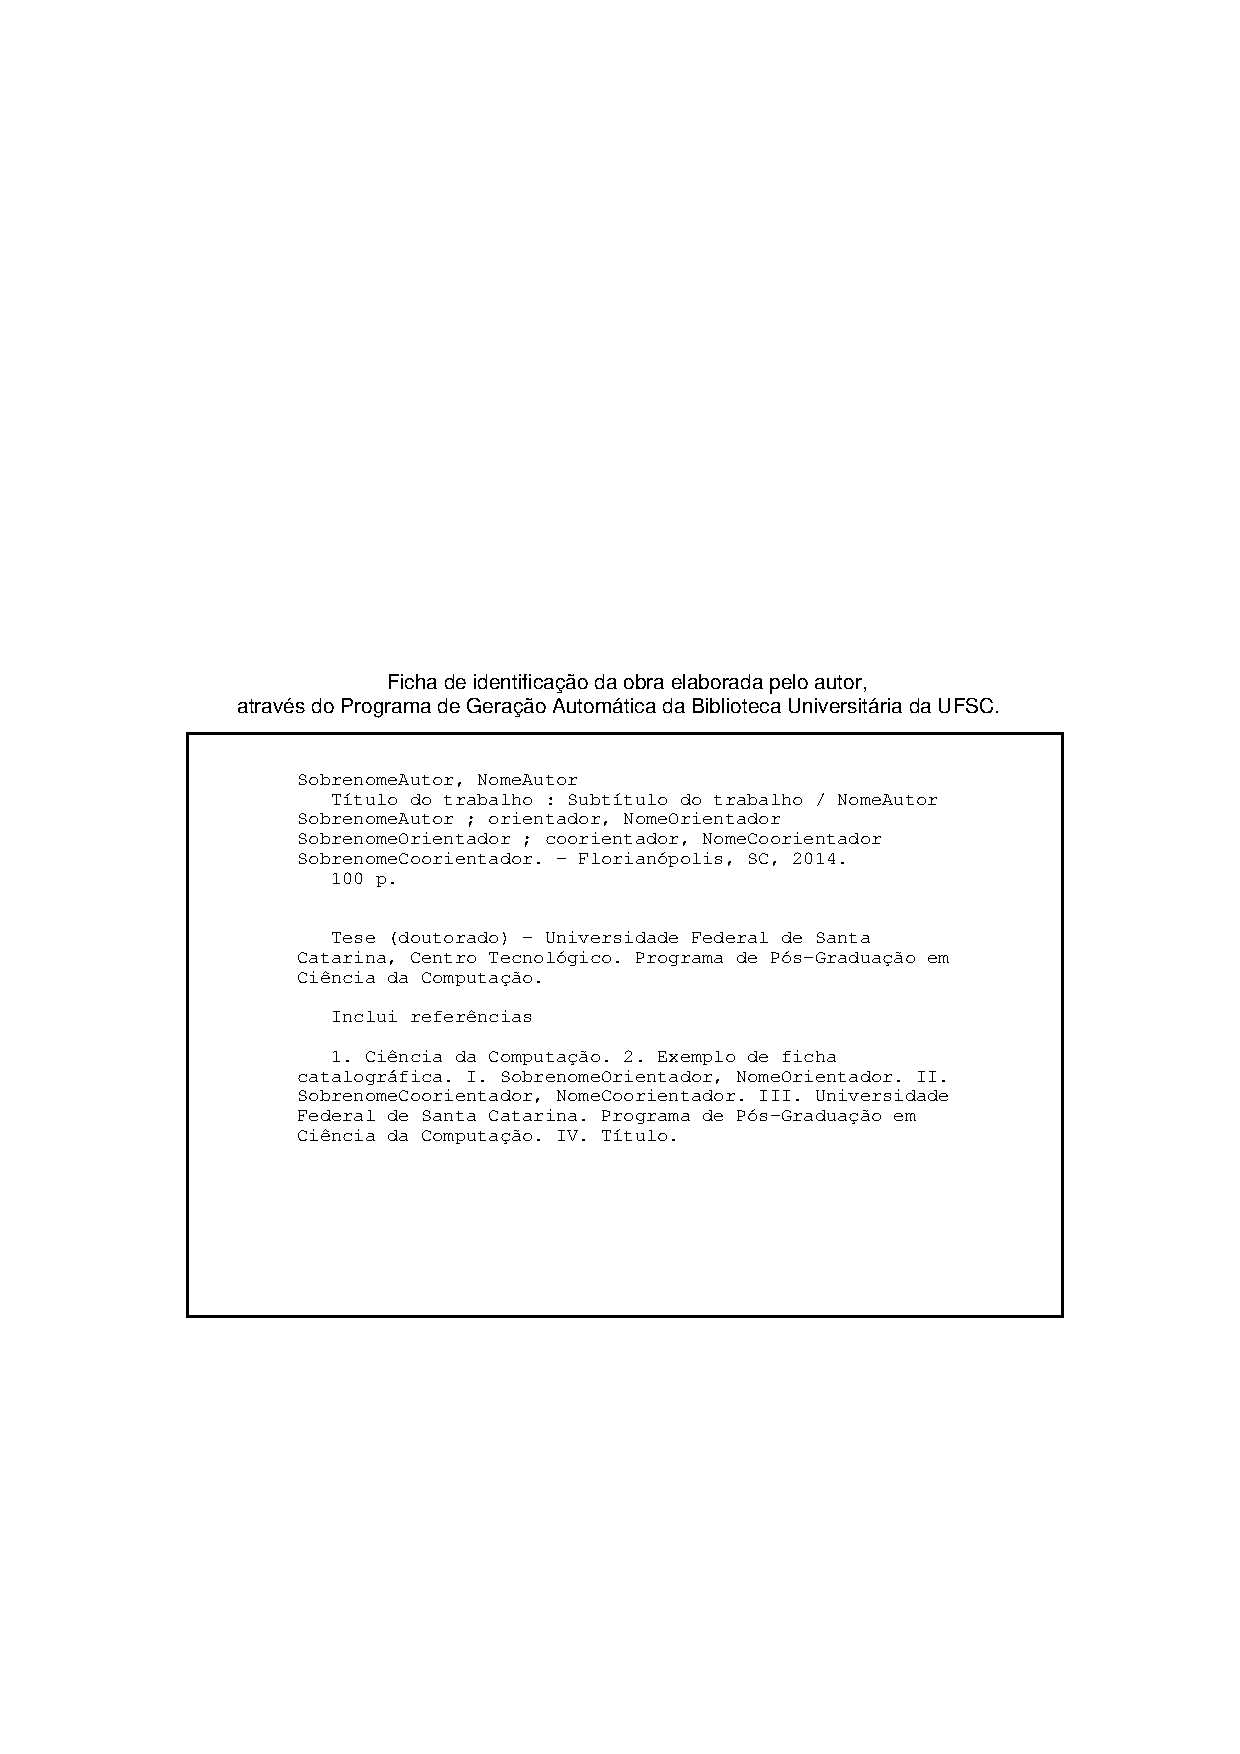
\includepdf{Ficha_Catalografica.pdf}
%\folhaderosto[comficha] % Se nao quiser imprimir a ficha, é só não usar o parâmetro
\folhaaprovacao
\paginadedicatoria
\paginaagradecimento
\paginaepigrafe
\paginaresumo
\paginaabstract
%\pretextuais % Substitui todos os elementos pre-textuais acima
\listadefiguras % as listas dependem da necessidade do usuário
\listadetabelas 
\listadeabreviaturas
\listadesimbolos
\sumario
%--------------------------------------------------------
% Elementos textuais

\chapter{Introdução}
Nos últimos 40 anos existiram varias predições para o futuro da humanidade, conceitos como IoT(\textit{Internet Of Things})\cite{gates1995estrada} e ambiente ubíquo\cite{weiser1991computer} foram criados, propostas tecnológicas como a \textit{lei de Moore}\footnote{Citação famosa utilizada por Gordon Earle Moore, que tinha como proposta a duplicação do numero de transistores a cada 18 meses} eram ditas como garantidas pelas grandes empresas de tecnologia. Contudo muitos desafios acabaram prejudicando a execução destas predições, como, por exemplo, a barreira de potência\cite{Patterson:2008:COD:1502247} e a limitação de densidade energética\cite{paradiso2005energy}.
%http://www.singularity.com/charts/page70.html

Hoje, o avanço tecnológico permitiu a miniaturização dos processadores com um custo de aquisição de grandezas menores das décadas anteriores\cite{nordhaus2007two}, possibilitando a pequenas empresas e até mesmo pessoas comuns o acesso a sistemas computacionais com alto processamento. Contudo, mesmo	 sendo possível, as ferramentas existentes para permitir o desenvolvimento de aplicações pros processadores, são geralmente pagas (\textit{IAR Embedded Workbench}\footnote{Não existe versão gratuita\cite{buyiar}.}), limitadas (\textit{MDK Microcontroller Development Kit}\footnote{Versão gratuita com limite de código de 32 Kbytes.}) ou com poucos recursos (\textit{Platformio}\footnote{Sem depuração embutida.}).
%http://www2.keil.com/mdk5

A comunidade dos desenvolvedores de software para sistemas embarcados tende a utilizar inúmeras ferramentas para resolver os desafios de projeto, geralmente embutidas em uma IDE (\textit{Integrated Development Environment}), permitindo funções básicas, por exemplo, depuração, comunicação, gravação, entre outros. Algumas IDEs tendem a resolver mais de um problema ao mesmo tempo, resultando num sistema complexo, abstraindo os sistemas que executam em segundo plano, resultando num uso maior do processador da maquina de trabalho, dificultando a personalização do fluxo de desenvolvimento e dos sistemas utilizados pelo desenvolvedor.

\iffalse
O intuito deste trabalho é a realização de um sistema para possibilitar aos desenvolvedores a programação de sistemas embarcados, sem a necessidade de utilizar sistemas assistencialistas que possam limitar a evolução do trabalho ou a utilização do produto final concebido.
\fi

\section{Motivação}

Com o avanço tecnológico e a evolução do hardware heterogêneo (sistemas com GPU (\textit{Graphic Processor Unit}), CPU (\textit{Central Processor Unit}) e outros periféricos), muitos dos sistemas disponíveis para desenvolvimento não seguem um padrão estabelecido no carregamento de código (gravador, protocolo, \textit{bootloader} e etc.), além disso, as empresas acabam criando alternativas aos padrões já
%https://community.nxp.com/thread/389162
 existentes no mercado ou opções limitadas nas IDEs, como, por exemplo, DebugWire\cite{debugwire}, hardware exclusivo de depuração LPC\cite{nxp}, suporte limitado de depuradores\cite{kiledebug} entre outros, dificultando ou restringindo o desenvolvimento do usuário.

Geralmente, as ferramentas utilizadas para o desenvolvimento são de código fechado, distribuídas numa versão binaria, restringindo a modificação do software pelo usuário e personalizações do desenvolvimento. No desenvolvimento do estado da arte, a personalização da ferramenta é essencial para permitir o desenvolvimento, evitando a espera do suporte dentro dos sistemas vendidos, desta forma, muitas empresas acabam aderindo aos software de código aberto pela sua agilidade para adesão a novas tecnologias, podendo destacar Microsoft\cite{microsoftn1}, Intel, Samsung, IBM e Renesas\cite{topskernel}.

\iffalse
\subsubsection{Ferramentas proprietárias}

Pela falta de um padrão definido, muitas empresas resolveram criar seus próprios, fundamentados em seus interesses ou na suas definições de utilização do que deveria ou não conter em suas soluções. Como consequência disso, são criados visões limitadas da realidade, resultante do modo de atuação interno vivida pela empresa, pela sua falta de conhecimento da realidade atual do mercado e suas utilizações.

Como consequência disso, a gama de padrões de protocolos de comunicação, \textit{bootloaders}, ICSPs, compiladores e outros materiais utilizados no desenvolvimento de sistemas embarcados, dificulta a realização do trabalho do desenvolvedor, principalmente se tais periféricos utilizados tem documentação e código fonte fechados, não permitindo seu conhecimento de funcionamento.
\fi
%\itodo{Adicionar footnote the bootloader}
%\subsubsection{Padronização}

\section{Objetivo Geral}


%comment
\iffalse
O objetivo geral deve responder as seguintes perguntas:
1) O que a sua organização deseja realizar com o Projeto?
2) Qual problema em especial se quer solucionar?
3) Que mudanças se quer alcançar?
4) Que diferença o projeto quer fazer?

Deve ser escrito em tempo infinitivo (por exemplo: ampliar, capacitar, entre outros) e redigido com claridade. O objetivo precisa ser alcançável, não pode ser genérico, de forma que o projeto não consiga resolver (ex: terminar com a fome no mundo). Por outro lado deve ser ousado, capaz de sinalizar mudanças mais profundas que poderão ser alcançadas pelo projeto a médio e longo prazo.
\fi

\subsection{Metodologia}
\label{ss:objetivosespecificos}
Para realizar os objetivos, os seguintes passos são listados:
\begin{enumerate}
\item Estudo inicial das ferramentas utilizadas para desenvolvimento de sistemas embarcados.
\item Escolha das ferramentas inicialmente suportadas.
\item Analise inicial sobre KDevelop.
%\footnote{adicionar nota de roda pé sobre o KDevelop, botar isso onde primeiramente acontece.} no irc \itodo{Adicionar abreviatura de irc} \footnote{Adicionar footnote sobre irc}.
\item Estudo para traçado inicial de estrutura e objetivo.
\item \textbf{Inicio do desenvolvimento}.
\item Carregamento do plugin.
\item Selecionar primeiro sistema embarcado para desenvolvimento.
\item Desenvolvimento do instalador de dependências.
\item Desenvolvimento de interface de programação.
\item Realização de testes utilizando o sistema selecionado.
\item Aprimoramento do sistema.
\item Selecionar outro sistema sistema embarcado para realizar o desenvolvimento.
\item Atualização do sistema de instalação.
\item Repetir passo 10 em diante.
\end{enumerate}

\section{Analise do fluxo de trabalho}

A interface de projeto existente no KDevelop, permite que boa parte das especificações de projeto fiquem no sistema de geração automatizada\footnote{Entre eles pode se destacar os mais utilizados são o \textit{Makefile}, \textit{CMakefile} e \textit{WAF}.}, permitindo o desenvolvimento de software sem a integração do projeto com o KDevelop para sua utilização.
\iffalse
, utilizando arquivos intermediários de configuração\footnote{Arquivos que contem informações sobre compilador, estilo de código, execução e etc.}.
\fi
Esta flexibilidade de integração de projetos no KDevelop acrescenta um grau de dificuldade na realização do plugin, pois, as informações necessárias no carregamento do binário para o sistema embarcado necessita de sua localização e da porta de comunicação para o hardware em desenvolvimento. %\itodo{ADICIONAR MAIS INFORMAÇÕES DE FLUXO}

\section{Estrutura do Trabalho}

\begin{enumerate}
\item \textbf{Introdução} - Tema e contextualização do que será abordado no trabalho.
\item \textbf{Fundamentos teóricos} - Revisão dos assuntos abordados e necessários, fundamentais para realização do projeto.
\item \textbf{Estado da arte} - Comparação dos sistemas existentes que abordam o assunto e tentam aplicar uma proposta de solução.
\item \textbf{Projeto da ferramenta} - Rascunhos iniciais de interface e arquitetura de software.
\item \textbf{Desenvolvimento} - Relato do trabalho realizado, contendo informações do projeto e seu andamento.
\item \textbf{Experimento e resultados} - Exposição dos resultados.
\item \textbf{Conclusão} - Conclusões finais.
\end{enumerate}
%\itodo{Expandir de forma mais detalhada}

\chapter{Fundamentos teóricos}

O desenvolvimento para sistemas embarcados necessita de uma interface para desenvolvimento do código fonte, um compilador para geração do código fonte para código de maquina e um sistema de carregamento do código de maquina para o sistema embarcado.

\section{Sistema embarcado}

Numa visão mais ampla, o sistema embarcado pode ser resumido para qualquer sistema que realiza uma tarefa especifica, independe do custo energético ou computacional\cite{barr2006programming}. Dentro desta categoria, pode-se listar alguns exemplos:

\begin{itemize}
\item \textbf{VANT} (Veículo Aéreo Não Tripulado) - Com crescimento exponencial nos últimos anos, atualmente se encontra com inúmeras propostas em suas utilizações.
\item \textbf{Roteador} - Extremamente populares no acesso da internet. Muitos contem uma arquitetura computacional completa , processador, memória e sistema operacional como o \textit{OpenWrt}\cite{openwrt}.
\item \textbf{GPS} (\textit{Global Positioning System}) - Com um sistema de processamento, podendo realizar filtragem, fusionamento, estimação e comunicação em inúmeros protocolos.
\item \textbf{Televisões} - Os modelos dos últimos anos tiveram como foco principal a extensão da televisão como ambiente de entretenimento, permitindo conexão com internet, instalação de aplicativos e serviços online de entretimento e informação.
\item \textbf{Câmeras de vigilância} - Alguns tipos permitem o acesso via internet, utilizando uma eletrônica embarcada com sistemas operacional e periféricos de rede.
\end{itemize}

\abreviatura{VANT}{\textit{Veículo Aéreo Não Tripulado}}
\abreviatura{GPS}{\textit{Global Positioning System}}

As definições de sistemas embarcados foram modificadas ao passar do tempo, como, por exemplo, o baixo processamento, que se tornou inapropriada ao passar dos anos\cite{aiimpacts}.

\iffalse
A evolução do hardware, diminuiu o tamanho e preço de aquisição dos processados, permitiu praticamente a qualquer desenvolvedor de
sistemas computacionais embarcados, um poder de processamento grande o suficiente para rodar um kernel\footnote{Cerne do sistema
operacional, tendo como principal função o escalonamento de tarefas e abstração dos periféricos de hardware utilizados da maquina,
como, por exemplo: placa de rede, sensores, portas de comunicação, \textit{GPIOs} e etc.} de sistema operacional complexo, como o Linux, em praticamente qualquer aplicação.

Muitas das aplicações de sistemas embarcados são utilizados para sistemas cyber-físicos\footnote{Sistemas computacionais
voltados para interação no mundo físico via atuadores e tendo como entrada informações de transdutores, alguns exemplos
podem se destacar: Controle de combustível, controladora de VANTs, impressora 3D e etc.}
\fi

\section{Distinção entre sistemas}
Dentro da área de sistemas embarcados, por envolver uma ampla gama de periféricos, utilizações, finalidades, pode-se resumir a certas categorias de destaque em relação a unidade principal de processamento, podendo destacar:

\subsection{Microcontrolador}

Um microcontrolador é definido como um sistema completo, sendo geralmente autossuficiente em relação aos periféricos necessários para realizar seu funcionamento. O processador, memória, periféricos de entrada e saída (\textit{ADC}, \textit{PWM}, \textit{GPIO}, entre outros) e oscilador na mesma pastilha de silício (\figref{fig:ricv}), barateando os custos de sua confecção, permitindo a popularização dos mesmos na industria e na comunidade DIY (Do It Yourself)/Makers\footnote{Cultura de desenvolvimento tecnológico próprio, derivado do movimento \textit{DIY}, sendo conhecido pela construção, modificação e manutenção pessoal.}. Estes mesmos
sistemas permitem o uso de osciladores externos, possibilitando o aumento da frequência de \textit{clock}\footnote{Sinal temporal periódico que determina a atualização dos registrados do sistema.} e como consequência um acréscimo no MIPS.

\abreviatura{DIY}{\textit{Do It Yourself}}
\abreviatura{SoC}{\textit{System on a chip}}
\abreviatura{ADC}{\textit{Analog to Digital Converter}}
\abreviatura{PWM}{\textit{Pulse Width Modulation}}
\abreviatura{GPIO}{\textit{General Purpose Input/Output}}
\abreviatura{DIY}{\textit{Do It Yourself}}
\abreviatura{MIPS}{Milhões de Instruções Por Segundo}

%https://twitter.com/onchipUIS/status/764289155983675392

\begin{figure}[!htb]
  \centering
  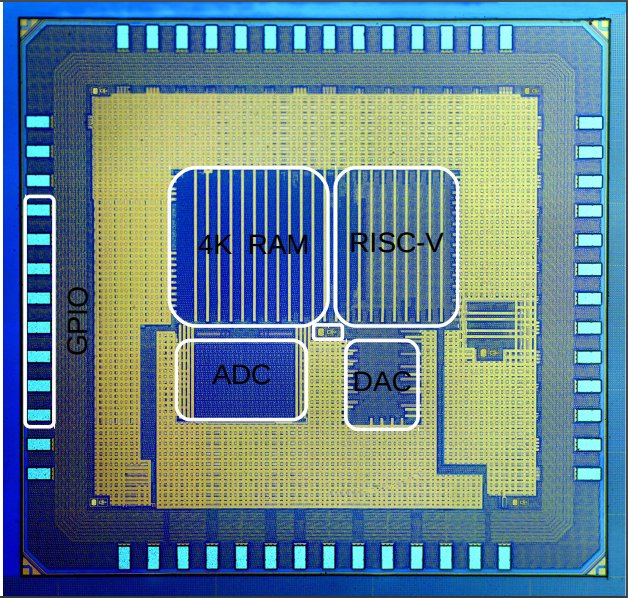
\includegraphics[width=0.5\textwidth]{figuras/riscv.jpg}
    \caption[Microcontrolador na pastilha de silício.]{Microcontrolador 32 bits baseado na arquitetura \textit{RISCV} (\textit{Reduced Instruction Set Computing - V})\footnote{Arquitetura aberta baseada na \textit{RISC}.}
  com periféricos (\textit{ADC}, \textit{DAC} (\textit{Digital-to-Analog Converter}), \textit{GPIO} e memória \textit{RAM} (\textit{Random Access Memory})), Fonte: onchip\cite{onchip}.}
  \label{fig:ricv}
\end{figure}

\abreviatura{DAC}{\textit{Digital-to-Analog Converter}}
\abreviatura{RAM}{\textit{Random Access Memory}}
\abreviatura{RISCV}{\textit{Reduced Instruction Set Computing - V}}

Se nas ultimas décadas, o acesso a computadores se tornou facilitado, nas próximas que estão por vir, o uso e aquisição de sistemas computacionais não será um mero luxo, mas sim uma inevitabilidadea\cite{gates1995estrada}. Tudo terá um processador, se não, um sistema computacional simples. Pode-se notar muitas etiquetas de RFID (\textit{Rafio Frequency Identification}) e cada vez mais modernas \cite{ricci2008design}, contendo sistemas computacionais complexos.

\abreviatura{RFID}{\textit{Rafio Frequency Identification}}

\subsection{Microprocessador}

Parte principal de um sistema computacional, com o objetivo de decodificar e executar as instruções em código de maquina existente na memória\cite{Patterson:2008:COD:1502247}. A tabela que é interpretada, denominada por conjunto de instruções, contem todos os padrões binários possíveis a serem decodificados, resultando em sinais lógicos para a eletrônica que o executará, podendo realizar comparações, somas, multiplexações e leituras/escritas na memória.

Com o passar dos anos, o poder de processamento permitiu que sistemas simples possam ter grande valor intelectual agregado, podendo utilizar como exemplo o termostato da Google, vendido atualmente por \$250, por realizar um \textit{aprendizado de maquina}\footnote{"Campo de estudo que dá aos computadores a habilidade de aprender sem serem explicitamente programados`` -  Arthur Samuel, 1945.}, proporcionando ao aparelho um melhor gerenciamento da temperatura do ambiente, realizando uma economia energética e uma melhora na qualidade de vida do usuário.

\subsection{SoC}

Atualmente o termo é empregado a circuitos com uma vasta quantidade de sistemas integrados, podendo citar  \textit{GPU} (\textit{Graphics Processing Unit}), \textit{USB} (\textit{Universal Serial Bus}), módulos de rede, rádio e outros sistemas mais avançados.

\abreviatura{GPU}{\textit{Graphics Processing Unit}}
\abreviatura{USB}{\textit{Universal Serial Bus}}

Nesta categoria, pode-se destacar o desenvolvimento dos sistemas desenvolvidos pela fabricante ARM, tendo ultrapassado a Intel como a maior produtora de processamentos do mundo.
Após a revolução dos dispositivos móveis onde a maioria das pessoas começaram a utilizar \textit{smartphones}, acarretando na substituição do uso de computadores para realizar as suas rotinas pessoais digitais diárias. Esta revolução, está fazendo uma grande modificação no ambiente de desenvolvimento das grandes empresas, permitindo o desenvolvimento de hardware sem a necessidade de empresas altamente especializadas para desenvolvimento, tornando um foco de desenvolvimento genérico e macroscópico.


\section{Bootloader}

A vantagem de se utilizar um sistema de carregamento de boot\footnote{Processo no qual o sistema computacional se inicia.} é
a gravação do programa principal com a assistência de um software primário, conhecido como \textit{bootloader}. Um microcontrolador
com este sistema, também pode ser denominado de auto-programável, pois possui as dependências necessárias para realizar o próprio
processo de programação.

Para entender melhor o funcionamento, pode-se utilizar uma maquina de estados para detalhar o \textit{bootloader} utilizado nos microcontroladores AVR (\figref{fig:sm_bootloader}), e uma descrição dos estados na \tabref{tab:bootloader}.

\begin{figure*}[ht!]
  \centering
  \begin{tikzpicture}[->,>=stealth',shorten >=1pt,auto,node distance=2.8cm,
                      semithick]
    \tikzstyle{every state}=[fill=blue,draw=none,text=white]

    \node[inicio,state]  (A)                    {$init\_hw$};
    \node[state]         (B) [right of=A]       {$new\_prg$};
    \node[state]         (C) [below of=B]       {$get\_com$};
    \node[state]         (D) [left of=C]        {$chk\_com$};
    \node[state]         (E) [left of=D]        {$exe\_com$};
    \node[state]         (F) [right of=B]       {$run\_prg$};

    \path (A) edge              node {}      (B)
          (B) edge              node {sim}   (C)
              edge              node {não}   (F)
          (C) edge              node {}      (D)
          (D) edge              node {correto}      (E)
              edge [bend right] node [above] {erro} (C)
          (E) edge [bend right] node [below] {}     (C);
  \end{tikzpicture}
  \caption[Máquina de estados do avr \textit{bootloader}]{\label{fig:sm_bootloader}}{Máquina de estados
  do avr \textit{bootloader},\\Fonte: \textit{AVR109: Self Programming - ATMEL}.}
\end{figure*}

\begin{table}[ht!]
\centering
\caption[Descrição dos estados do \textit{bootloader}]{Descrição dos estados da \figref{fig:sm_bootloader}}
\label{tab:bootloader}
\begin{tabular}{@{}l l p{55mm}@{}}
\toprule
Estado             & Próximos estados           & Descrição                                                                                                             \\ \midrule
\textit{init\_hw}  & \textit{new\_prog}         & Inicializa depêndencias de hardware para a utilização do \textit{bootloader}, Ex: serial.                \\
\textit{new\_prog} & \textit{get\_com,run\_prg} & Espera uma interrupção de hardware ser inicializada para inicialização da rotina de \textit{bootloader}. \\
get\_com           & \textit{chk\_com}          & Adiquiri os dados do \textit{buffer} da serial.                                                                     \\
chk\_com           & \textit{exe\_com,get\_com} & Checa o comando recebido pela serial, caso o não é valido outro comando deverá ser buscado.                           \\
exe\_com           & \textit{get\_com}          & Executa o comando após a validação                                                                                    \\
run\_prg           &                            & Inicializa programa principal caso a rotina de programação não é inicializada via interrupção de hardware. \\ \bottomrule
\end{tabular}
\end{table}

O \textit{bootloader}, por ser uma peça de software essencial dos sistemas auto-programáveis, ele se encontra na parte da memória
não volátil, existindo dentro de uma faixa determinada da memória ao lado do programa principal que será executado, como pode ser
visualizado na \figref{fig:me_bootloader}.

\begin{figure*}[ht!]
  \centering
  \begin{bytefield}{11}
    \memsection{ffff ffff}{002f c000}{6}{Pilha}\\
    \begin{rightwordgroup}{Flash}
        \memsection{002f bfff}{0001 0000}{3}{Aplicação principal}\\
        \memsection{0000 ffff}{0000 0000}{2}{\textit{Bootloader}}
    \end{rightwordgroup}\\
  \end{bytefield}
  \caption[Memória com \textit{bootloader}]{\label{fig:me_bootloader}}{Memória com \textit{bootloader},\\Fonte: 
  \textit{``Modular bootloader framework for silicon labs SIMXXXXX microcontrollers - Silicon Labs''}.}
\end{figure*}

%\subsection{Gravação}
%O processo é a transmissão do novo código a ser enviado para a memória do sistema embarcado, r

%\itodo{[ADICIONAR  UMA LISTA DOS BOOTLOADERS]}

\section{Programação externa}
%é importante
A realização da programação externa, utilizando um hardware especializado que  permiti a programação do processador, independente do software que já está programado ou em execução.
Alguns processadores, que se encontram em estados indevidos ou não planejados, podendo acarretar no mal funcionamento do sistema, podem ser regravados sem a preocupação do \textit{bootloader}, utilizando a gravação com a ferramenta do hardware especializado, limpando toda a memória e gravando o programa. O mesmo também é necessário para realizar a gravação do \textit{bootloader} pela primeira vez no processador, após isso, o próprio \textit{bootloader} pode se reprogramar ou atualizar.

A programação via um hardware especializado é geralmente concebida, dentro dos softwares livres, com o OpenOCD (\textit{Open On Chip Debugger})\cite{openocd}, realizando a interface de software na comunicação com o hardware especializado como o JTAG (\textit{Joint Test Action Group}).

\abreviatura{JTAG}{\textit{Joint Test Action Group}}
\abreviatura{OpenOCD}{\textit{Open On Chip Debugger}}

\subsection{JTAG}

Com o avanço na miniaturização dos circuitos integrados e o aumento da densidade de componentes nos circuitos impressos, foi necessária o desenvolvimento de novos métodos para realização de testes de integridade.

Para superar esse problema, os maiores fabricantes de componentes combinaram por uma forma conhecida como JTAG, resultando no padrão IEEE (\textit{Institute of Electrical and Electronic Engineers}) 1149.1 \cite{jtagcite}.

O JTAG comunica principalmente com dois tipos de registradores, o registrador de instruções e os registradores de dados.

\begin{itemize}
\item \textbf{Registrador de instrução}: Tem em seu conteúdo a instrução que está sendo executada no momento pelo processador.
\item \textbf{Registrador de dados}: Na categoria de registrador de dados, o JTAG utiliza três tipos.
\subitem BSR (\textit{Boundary Scan Register}): Utilizado para mover os dados dos estados de I/O (\textit{Input/Output}).
\subitem BYPASS: Registrador de 1 bit utilizado para selecionar o hardware testado.
\subitem IDCODES: Contem as informações sobre o hardware em analise (ID, revisão entre outros), podendo conduzir ao JTAG a configuração para o hardware.
\end{itemize}

\subsection{OpenOCD}

Realizar a depuração do hardware é diferente de uma aplicação comum, o código é executado em um sistema limitado, podendo não ter o suporte para logs, despejo de memória entre outros.

Utilizando o JTAG, é possível ter acesso aos estados dos pinos, memó-\\ria e instruções em execução. Para visualizar e interpretar os dados recebidos do JTAG, é geralmente utilizado uma ferramenta conhecida como GDB (\textit{GNU Project debugger}). Contudo, para a comunicação do computador com o JTAG, realizando a depuração do sistema embarcado, é utilizado outro software, providenciando uma camada de abstração para o GDB via o protocolo do \textit{gdbserver}, como o \textit{OpenOCD} (Algoritmo 2.1). Este é mantido pela comunidade de código aberto, tendo um suporte a uma vasta gama de JTAGs.

\lstinputlisting[caption={[Resultado]OpenOCD respondendo ao GDB},name=teste]{openocd.txt}

\section{KDevelop}
O plugin proposto foi desenvolvido sobre a plataforma conhecida como KDevelop,\cite{kdevelop} pertencente a organização \textit{KDE},
sendo um conceito de \textit{IDE} para programação.

Concebido utilizando as tecnologias de código aberto mais modernas, como C++14, QT 5.8, entre outras bibliotecas e ferramentas
utilizadas, podendo assim denominar o sistema como \textit{Rolling release}\footnote{Sistemas de software que atualizam suas bases
de código para a utilização das ultimas versões das ferramentas empregadas no projeto.}.

O KDevelop teve seu primeiro lançamento em 1999, sendo majoritariamente programado em C++, podendo ser utilizado
para programar em C, C++, Perl, Python, PHP, Java, Fortran, Ruby, Ada, Pascal, SQL e Bash. Suportando também sistemas de
configuração para compilação como cmake, qmake e make.

Diferente de outras \textit{IDEs} que propõem as mesmas soluções que o KDevelop, este é inteiramente desenvolvido
com foco em performance e numa agradável experiência do usuário, permitindo o desenvolvimento e adesão de projetos na \textit{IDE} (\textit{Integrated Development Environment}) sem restringir outros ambientes de desenvolvimento, utilizando toda a informação disponível nos sistemas assistencialistas de configuração de compilação, como fonte das dependências e de informações sobre o projeto adicionado. Para um programador comum de código aberto, o KDevelop se apresenta como uma ótima opção.

\abreviatura{IDE}{\textit{Integrated Development Environment}}

\subsection{Plugins}
O \textit{plugin} opera como uma biblioteca compartilhada que é carregada durante o tempo de execução, desta forma, providenciando acesso as funções da biblioteca. Uma grande vantagem da sua utilização é o uso modular das dependências utilizadas no projeto, sem a necessidade de ter o conjunto como um único binário com todas as dependências, mesmo aquelas não utilizadas pelo desenvolvedor.

Uma outra vantagem da utilização de \textit{plugins}, é permitir somente a utilização do binário, sem a necessidade de utilizar
o código fonte do mesmo, permitindo, a utilização de \textit{plugins} que não são de código aberto, facilitando desta
forma o apoio e uso de sistemas proprietários desenvolvidos, mantendo sigiloso o trabalho intelectual.

\section{Tipos de ferramenta}
Das ferramentas disponibilizadas para o desenvolvimento destas a Plicações possuem algumas limitações tais como, preço, licença, configuração entre outros, podendo ser classificadas conforme as seguintes categorias:

\begin{itemize}
 \item \textbf{Ferramentas proprietárias}: Ferramentas de desenvolvimento que geralmente utilizam software e hardware desenvolvido pelo próprio fabricante, não dando suporte a outros periféricos que não pertencem a mesma distribuidora ou parceira, limitando a liberdade de desenvolvimento. Outras permitem o desenvolvimento limitado para cada tipo de licença, dificultando o desenvolvimento que utilizam baixo orçamento, como, por exemplo: Limitação de tamanho de código\cite{simplicity}, pagar uma licença mais cara para utilizar opções de compilação otimizada (-O2 e -OS do GCC, C++11/14)\cite{armdeveloper} ou até mesmo opções para utilizar o algumas partes do processador (neon, -mfloat-abi e -mfpu dos processadores ARM, permitindo execução de cálculo matricial ou com ponto flutuante em hardware)\cite{neon}. A utilização de ferramentas proprietárias são majoritariamente usadas.

 \item \textbf{Ferramentas de código aberto}: Utilizadas por uma parte dos desenvolvedores, fornece acesso total as suas funcionalidades, possibilitando modificações e aperfeiçoamentos nos mínimos detalhes. Estas interfaces permitem o desenvolvimento com uma experiência mais assistencialista, por possuir uma comunidade grande de desenvolvedores que disponibiliza suporte por e-mail ou grupos de chat. Contudo, por estar em constante evolução, sua documentação pode estar defasada ou inexistente.

\end{itemize}

\section{Sistema de Controle de Versão}

Para o controle do projeto desenvolvido foi utilizado o \textit{GIT}, permitindo o controle de versão do código, paralelismo no desenvolvimento, detecção de conflitos entre diferentes versões, detecção de erros, entre outras utilizações de grande valia
para o desenvolvimento de software.

\abreviatura{GIT}{\textit{Global Information Tracker}}


\chapter{Estado da Arte}
As interfaces mais populares para desenvolvimento em sistemas embarcados são majoritariamente desenvolvidas sobre interfaces de programação genéricas e utilizadas para os mais variados fins, e dentre estas, muitas são desenvolvidas utilizando a linguagem de programação JAVA, conhecida por ser uma linguagem de baixo desempenho por ser executado pela JVM (\textit{Java Virtual Machine}).

\abreviatura{JVM}{Java Virtual Machine}

Boa parte destas IDE são de código fechado, com certas restrições para o desenvolvedor, restringindo a liberdade do mesmo no seu fluxo de trabalho, em alguns casos obrigando a utilizar hardwares proprietários para a execução de tarefas voltados a sistemas embarcados, obrigando a empresa ou usuário adquirir soluções desenvolvidas pelos fornecedores. Alem disso, tais sistemas profissionais são conhecidos por terem preços desproporcionais as suas funções comparadas as alternativas de código aberto, podendo custar até milhares de dólares %\itodo{[ACHAR A FONTE DISSO AQUI]}.

Dentro das opções de código aberto de desenvolvimento de sistemas embarcados, pode-se se destacar a Arduino, que disponibiliza tanto o software quanto o hardware. A sua popularidade veio como consequência da sua cultura de desenvolvimento de \textit{Open Source}, onde tanto o hardware, quanto o software distribuídos tem sua documentação por completo aberta, permitindo que inúmeros entusiastas desenvolvam sem a necessidade de restrições, muitos outros acabam colaborando com os próprios projetos da empresa, facilitando desta forma o trabalho da mesma, produzindo versões melhoradas de seus produtos com a ajuda dos próprios usuários e suas contribuições. A IDE desenvolvida pela Arduino e concebida majoritariamente em JAVA.

Outras duas interfaces de código aberto utilizadas para sistemas embarcados são Eclipse e CCS, sendo o segundo baseado no primeiro
derivado pela empresa conhecida como \textit{Texas Instruments}. Baseados na linguagem de programação JAVA, possibilitam uma
integração com plugins relativamente fácil, podendo ser expandidas de acordo com o desenvolvedor e a disponibilidade das mesmas.

\section{IDE Existentes}
Dentro das opções disponíveis, pode-se destacar (Tabela \ref{ides}):
%\itodo{[EXPANDIR DESCRIÇÃO]}
\iffalse
\begin{itemize}
 \item \textbf{Atmel Studio}
 \subitem Limitado aos processadores AVR.
 \subitem Código fechado.
 \subitem Preço: Pago.

 \item \textbf{Arduino IDE}
 \subitem Limitado ao suporte para placas da mesma plataforma com processadores AVR e ARM, alem de algumas personalizadas
 pela comunidade open source, como, por exemplo: ESP-8266
 \subitem Código aberto.
 \subitem Preço: Grátis.

 \item \textbf{ArduIDE}
 \subitem Limitado aos processadores AVR.
 \subitem Código aberto.
 \subitem Preço: Gratuito.

 \item \textbf{PROGRAMINO IDE}
 \subitem Limitado aos processadores AVR.
 \subitem Código fechado.
 \subitem Preço: 30 euros.

 \item \textbf{PlatformIO}
 \subitem Plugin para Atom, que por sua vez é baseado em um browser.
 \subitem Código aberto.
 \subitem Preço: Gratuito.

 \item \textbf{Embrio}
 \subitem Limitado aos processadores AVR.
 \subitem Código fechado.
 \subitem Preço: 59 dólares.

 \item \textbf{Embedded Studio}
 \subitem Para fins educacionais, limitado aos processadores ARM.
 \subitem Código fechado
 \subitem Preço: Gratuito.

 \item \textbf{IAR}
 \subitem Limitado aos processador ARM.
 \subitem Código fechado.
 \subitem Preço: Pago.

 \item \textbf{mikroe IDE}
 \subitem Limitado aos processador ARM da família M3 e M4.
 \subitem Código fechado.
 \subitem Preço: 299 dólares.

 \item \textbf{GNU ARM Eclipse}
 \subitem Limitado aos processadores ARM, plugin para a IDE Eclipse.
 \subitem Código aberto.
 \subitem Preço: Gratuito.

 \item \textbf{CrossWorks}
 \subitem Depende do tipo de licença, limitado aos processador ARM.
 \subitem Código fechado.
 \subitem Preço: \$150 até \$2250.

 \item \textbf{Code Composer Studio}
 \subitem Dependendo do tipo de licença.
 \subitem Código fechado.
 \subitem Preço: Grátis até \$5495.
 
 \item \textbf{Keil}
 \subitem Dependendo do tipo de licença.
 \subitem Código fechado.
 \subitem Preço: Grátis até \$5495.
 
 \item \textbf{Simplicity-studio}
 \subitem Dependendo do tipo de licença.
 \subitem Código fechado.
 \subitem Preço: Pago.

\end{itemize}
\fi

% Please add the following required packages to your document preamble:
% \usepackage{booktabs}
\begin{table}[]
\centering
\caption{IDE existentes}
\label{ides}
\begin{tabular}{@{}llll@{}}
\toprule
Nome                  & Processadores                                          & Código  & Valor              \\ \midrule
ArduIDE               & AVR e ARM                                     & Aberto  & Gratuito           \\
Arduino IDE           & \makecell[l]{AVR, ARM, X86, espressif,\\RISCV entre outros.} & Aberto  & Gratuito           \\
Atmel Studio          & AVR                                           & Fechado & Pago               \\
Code Composer Studio  & \makecell[l]{ARM, DSP, TSM,  MSP\\entre outros.}                      & Fechado & Até 4500 dólares   \\
CrossWorks            & ARM                                                    & Fechado & 150 a 2250 dólares \\
EmbeddedStudio        & ARM                                                    & Fechado & Gratuito           \\
Embrio                & AVR                                                    & Fechado & 59 dólares         \\
GNU ARM Eclipse       & ARM                                                    & Aberto  & Gratuito           \\
IAR                   & \makecell[l]{AVR, ARM, X86,  MSP\\entre outros.}                      & Fechado & Pago  \\
Keil                  & \makecell[l]{ARM, X86, AVR\\entre outros.}                            & Fechado & Até 5495 dólares   \\
mikroe IDE            & ARM                                                    & Fechado & 299 dólares        \\
PlatformIO            & \makecell[l]{AVR, ARM, X86, espressif,\\RISCV entre outros.} & Aberto  & Gratuito           \\
PRAGRAMINO IDE        & AVR                                           & Fechado & 30 euros           \\
Simplicity Studio     & ARM, X86 entre outros.                                 & Fechado & Pago.              \\ \bottomrule
\end{tabular}
\end{table}

\newpage

Maioria das IDEs citadas são de código fechado e pagas, impossibilitando sua modificação. Dentre as gratuitas, a Arduino IDE e PlatformIO tem suporte para múltiplas arquiteturas, contudo, estas IDEs são limitadas no desenvolvimento ou na performance, contendo pouca ou nenhuma opção de \textit{code parsing}, gerenciamento de projeto, depuração, entre outros. É conclusivo que dentre as opções citadas nenhuma atende os requisitos do projeto, ressaltando a necessidade deste trabalho para a comunidade de desenvolvedores de sistemas embarcados.


\iffalse
\section{Dificuldades}
Pela constante evolução no mundo de sistemas embarcados, cada empresa acaba criando se próprio padrão de desenvolvimento para os
usuários, tendo o intuito de ajuda-los, acaba prejudicando o trabalho dos desenvolvedores com conhecimento avançado. Tal conhecimento não se trata de um arquitetura de hardware especifica, ou da abstração de software utilizada pelo fabricando para não resultar no uso de software a nível de registrador, mas sim o conhecimento sobre como o processo de gravação é realizado de forma intrínseca na visão de hardware e software integrados.

Boa parte das interfaces de programação para sistemas embarcados se trada de um sistema com vasta quantidade de configurações,
com uma quantidade de abas e janelas que tornar inusual a utilização do gerenciador de projeto. Mesmo o intuito do fabricante ser bom,
isso acaba torna os desenvolvedores escravas da ferramenta, sendo obrigados a conhecer todas as peculiaridades da mesma para a sua
utilização, fazendo com que a curva de aprendizado e desenvolvimento muito engrime.

Outro problema, é a falta de padronização entre os fabricante, nas placas de desenvolvimento, nos gravadores, nas IDEs e nas bibliotecas
básicas utilizadas para desenvolvimento do software de sistema embarcado. Atualmente, um dos padrões mais utilizados para software
de sistemas embarcados, são as nomenclaturas utilizadas pela Arduino e pelo CMSIS, o primeiro por ser o mais utilizado por hobbistas
e o segundo por ser o mais utilizado entre os desenvolvedores que optam pelos processadores derivados da arquitetura ARM.
\fi
\abreviatura{CMSIS}{Cortex Microcontroller Software Interface Standard}


%http://www.linux-magazine.com/Online/Blogs/Paw-Prints-Writings-of-the-maddog/Brazil-Free-and-Open-Source-Culture-Is-Economics-Not-Politics
%https://books.google.com.br/books?id=pxAVCgAAQBAJ&pg=PA166&lpg=PA166&dq=Brazil:+Free+and+Open+Source+Culture+Is+Economics,+Not+Politics&source=bl&ots=k5M51pGklX&sig=tCPn4l7OnL7Xzne9cKYowUbYTvo&hl=pt-BR&sa=X&ved=0ahUKEwihkIec0-HPAhUGjpAKHdv6AcwQ6AEIOzAE#v=onepage&q=Brazil%3A%20Free%20and%20Open%20Source%20Culture%20Is%20Economics%2C%20Not%20Politics&f=false
%http://pear.accc.uic.edu/ojs/index.php/fm/article/view/904/813
%https://books.google.com.br/books?id=fEP2smsHVCwC&pg=PA14&lpg=PA14&dq=Brazil:+Free+and+Open+Source+Culture+Is+Economics,+Not+Politics&source=bl&ots=FsxRuW6joV&sig=l_PNwCwjTLl-XBATmeSIVO70Fcs&hl=pt-BR&sa=X&ved=0ahUKEwihkIec0-HPAhUGjpAKHdv6AcwQ6AEISzAG#v=onepage&q=Brazil%3A%20Free%20and%20Open%20Source%20Culture%20Is%20Economics%2C%20Not%20Politics&f=false
\chapter{Projeto da ferramenta}

KDE é conhecido por utilizar as ferramentas e bibliotecas disponibilizadas pela \textit{QT Project}\footnote{Empresa desenvolvedora  de software, famosa pelas suas bibliotecas e \textit{IDEs} de desenvolvimento} para a realização do desenvolvimento dos seus projetos. O conhecimento inicial de como utilizar tais ferramentas é de grande valia para o projeto do desenvolvimento da proposta, principalmente pelo fato de se conhecer as possibilidades.


\section{Requisitos funcionais}

O usuário deve ser capaz de utilizar o plugin para realizar a programa-\\ção de sistemas embarcados, com a ajuda de um \textit{bootloader}, ou utilizando programadores direto no hardware. Além de ser possível programar, dependendo do caso, o desenvolvedor seria capaz de utilizar o plugin para a realização da depuração do projeto dentro do próprio sistema em desenvolvimento, caso o sistema utilizado por suportar tal comportamento.

A escolha do Arduino se deu ao fato pela sua fácil aquisição, baixo preço e popularidade dentre a comunidade civil como um dos microcontroladores mais populares, desta forma, seria um bom primeiro passo para a realização da estrutura de software a ser desenvolvida para o plugin.

O sistema deve ter as seguintes funcionalidades para exercer um bom funcionamento para o usuário.
\begin{itemize}
\item O sistema deve permitir ao usuário:
	\subitem A criação de novos projetos e disponibilizar um modelo.
	\subitem Integração de projeto do usuário.
    \subitem Configuração das ferramentas utilizadas.
	\subitem Executar a compilação do projeto.
	\subitem Executar a instalação de ferramentas.
	\subitem Carregar o binário para o sistema embarcado.
\item O projetos devem ser salvos assim como as configurações.
\item Executar o carregamento utilizando as ferramentas selecionadas.
\item Avisar sobre erros e problemas durante a ocorrência de alguma etapa para o usuário.	
\end{itemize}

\section{Requisitos não funcionais}
Algumas propriedades e restrições do sistema são vitais para seu funcionamento.
\begin{itemize}
\item O sistema deve executar sem acarretar numa falha ao execução.
\item A instalação de ferramentas devem ser feitas sem a permissão de administrador.
\item O programa deve executar sem vazamento de memória.
\item Durante a instalação das dependências, deve ser utilizado nomes randômicos durante o download por segurança, evitando a manipulação do arquivo por terceiros.
\end{itemize}

\section{Plataformas suportadas}

Neste projeto, como versão inicial, será suportado as plataformas mais populares da Arduino, validando o suporte para outras placas com processadores AVR, e os sistemas que utilizam \textit{OpenOCD}\footnote{utilizando majoritariamente em placas com processadores ARM (Arduino DUE, STM32, entre outros).}, outros suportes podem vir a ser adicionados em futuras versões.


%Em futuras versões mais  ferramentas deverão ser adicionados,
%, serão os primeiros a serem suportados pelo plugin como prova de conceito por apresentarem uma grande quantidade de usuários.
%Como objetivo final do projeto, o usuário deve ser capaz de utilizar o


\chapter{Desenvolvimento}

Diferente de muitas outras interfaces de desenvolvimento, o KDevelop permite ao usuário incorporar qualquer projeto de software na IDE, contanto que siga alguns padrões já estabelecidos. Boa parte das configurações utilizadas no projeto são oriundas dos gerenciadores de compilação, minimizando o trabalho do usuário.

\section{Ferramentas Utilizadas}
As seguintes ferramentas foram utilizadas para desenvolvimento do projeto.
\begin{itemize}
 \item \textbf{KDevelop}: Editor de código para desenvolvimento do plugin e na realização de debug.
 \item \textbf{QT Framework}: Kit de ferramentas e bibliotecas para desenvolvimento de software.
 \item \textbf{KDE Framework}: Coleção de ferramentas e bibliotecas do KDE.
 \item \textbf{Avrdude}: Programa de carregamento de código para microcontroladores AVR.
 \item \textbf{OpenOCD}: Ferramenta para comunicação de programadores.
 \item \textbf{Placas de desenvolvimento}: Arduino mini, nano, mega, due, uno para testes de suporte utilizando avrdude e Stellaris como EK-LM4F232 para testes utilizando o OpenOCD.
\end{itemize}

O trabalho segue a filosofia GNU \cite{filosofia}, onde, todas as ferramentas utilizadas para o desenvolvimento do plugin são de código aberto e totalmente gratuitas para qualquer um que queira replicar, modificar e contribuir com o projeto.


\subsection{Arduino \textit{toolkit}}
O Arduino \textit{toolkit} possui inúmeras bibliotecas e arquivos de configuração, contendo informações como \textit{bootloader}, configurações de registradores, pinos, funções, entre outros.

O \textit{toolkit} foi utilizado para extração das opções de configuração, podendo dar destaque ao arquivo \textit{boards.txt}.

\lstinputlisting[caption={Parte referente ao Arduino nano de boards.txt},label=boardstxt]{boards.txt}

Dentro deste arquivo se pode extrair várias informações pertinentes para o sistema.

\begin{itemize}
\item \textit{upload.tool} - Ferramenta para envio do código de máquina.

\item \textit{upload.protocol} - Protocolo de comunicação com o \textit{bootloader}.
%http://www.atmel.com/images/Atmel-8271-8-bit-AVR-Microcontroller-ATmega48A-48PA-88A-88PA-168A-168PA-328-328P_datasheet_Complete.pdf

%http://www.avrfreaks.net/forum/self-programming-and-lock-bits

\item \textit{bootloader.tool} - Ferramenta responsável pela comunicação com o \textit{bootloader}.

\item \textit{bootloader.unlock\_bits} - Bits para desbloquear o \textit{bootloader} na realização de escrita.

\item \textit{bootloader.lock\_bits} - Bits para bloquear o \textit{bootloader} na realização de escrita.
\subitem Tanto o \textit{unlock\_bits} quanto o \textit{lock\_bits} controla a programação externa como ISP (\textit{In-Circuit Serial Programmer}), JTAG, entre outros \cite{fuseSettings}. 
\abreviatura{ISP}{\textit{In-Circuit Serial Programmer}}

\item \textit{build.f\_cpu} - Clock do processador programado, configurado via \textit{bootloader}.

\item \textit{build.board} - Nome da placa.

\item \textit{build.core} - Tipo de hardware.

\item \textit{build.variant} - Topologia do hardware.

\item \textit{upload.maximum\_size} - Espaço livre na \textit{flash}, descontando \textit{bootloader}.

\item \textit{upload.maximum\_data\_size} - Espaço livre na \textit{RAM}.

\item \textit{upload.speed} - Velocidade da comunicação com o \textit{bootloader}.

%http://archive.fabacademy.org/archives/2016/doc/fuses.html
\item \textit{upload.low\_fuses}
\item \textit{upload.high\_fuses}
\item \textit{upload.extended\_fuses}
\subitem Bytes com memória não volátil do processador, conhecidos como \textit{low\_fuses}, \textit{high\_fuses} e \textit{extended\_fuses}. Estes são responsáveis por determinar o comportamento do processador. Podendo controlar o consumo energético, geração de clock, tempo de boot, tipo de clock, pino de reinicialização, modo de depuração, modo de programação, falhas de operação, monitor da tensão de alimentação, entre outros\cite{fuseSettings}\cite{fuses}.

\item \textit{upload.bootloader\_file} - Nome do arquivo que contem o código de máquina do sistema de \textit{bootloader}.

\item \textit{build.mcu} - Processador utilizado\cite{ATmega48A}.

\end{itemize}

Estas informações são de suma importância para a utilização da ferramenta de carregamento de código, \textit{avrdude}.

Nesta ferramenta, várias opções são necessárias para programar o sistema embarcado, dentro destas, pode-se destacar.

\begin{itemize}
\item \textit{partno} - Processador utilizado.

\item \textit{baudrate} - Velocidade de comunicação com o \textit{bootloader}.

\item \textit{config-file} - Arquivo de configuração do processador.

\item \textit{programmer} - Hardware utilizado para realizar o processo de gravação.

\item \textit{port} - Porta de comunicação com o hardware.

\item \textit{memtype} - Configuração da memória do processador.

\item \textit{filename} - Arquivo que contem o código de máquina.

\item \textit{U} - Além do \textit{memtype} e \textit{filename}, é possível passar o parâmetro \textit{U} junto com configurações de \textit{fuses} e \textit{lock/unlock} bits.
\end{itemize}

Para utilizar essas configurações é necessário um conhecimento do funcionamento do hardware e como essas opções afetam o sistema embarcado. 

\subsection{OpenOCD}

Recebe como argumentos os parâmetros de configuração ou comandos para a comunicação do JTAG. As opções disponíveis são:

\begin{itemize}
\item {file} - Aponta o arquivo de configuração.
\item {debug} - Nível da mensagem de depuração.
\item {command} - Executa um comando do OpenOCD.
\end{itemize}

Um exemplo de comando utilizado com a ferramenta, pode ser visto no Algoritmo \ref{openocdcli}, \ref{lm4f232cfg} e \ref{tiicdicfg}.

\lstinputlisting[caption={Linha de comando do OpenOCD},label=openocdcli]{openocdcli.txt}.

%%/usr/share/openocd/scripts/board/ek-lm4f232.cfg
\lstinputlisting[caption={board/ek-lm4f232.cfg},label=lm4f232cfg]{ek-lm4f232.cfg}

%/usr/share/openocd/scripts/interface/ti-icdi.cfg
\lstinputlisting[caption={interface/ti-icdi.cfg},label=tiicdicfg]{ti-icdi.cfg}

%/usr/share/openocd/scripts/target/stellaris.cfg

Onde \$\{bin\} é definido pelo caminho do arquivo de código de máquina e os valores de PID e VID pelo \textit{usbutils}.
Para criar o arquivo de configuração do OpenOCD, é necessário o conhecimento das características e do funcionamento do hardware.

\section{Fluxo de trabalho}

A interface de projeto existente no KDevelop permite que boa parte das especificações de projeto fiquem no sistema de geração automatizada\footnote{Entre eles pode se destacar os mais utilizados são o \textit{Makefile}, \textit{CMakefile} e \textit{WAF}.}, permitindo o desenvolvimento de software sem a integração do projeto com o KDevelop para sua utilização.
\iffalse
, utilizando arquivos intermediários de configuração\footnote{Arquivos que contem informações sobre compilador, estilo de código, execução e etc.}.
\fi
Esta flexibilidade de integração de projetos no KDevelop acrescenta um grau de dificuldade na realização do plugin, pois, as informações necessárias no carregamento do binário para o sistema embarcado necessita de sua localização e da porta de comunicação para o hardware em desenvolvimento. %\itodo{ADICIONAR MAIS INFORMAÇÕES DE FLUXO}

\section{Desenvolvimento do software}

\begin{figure}[!htb]
  \centering
  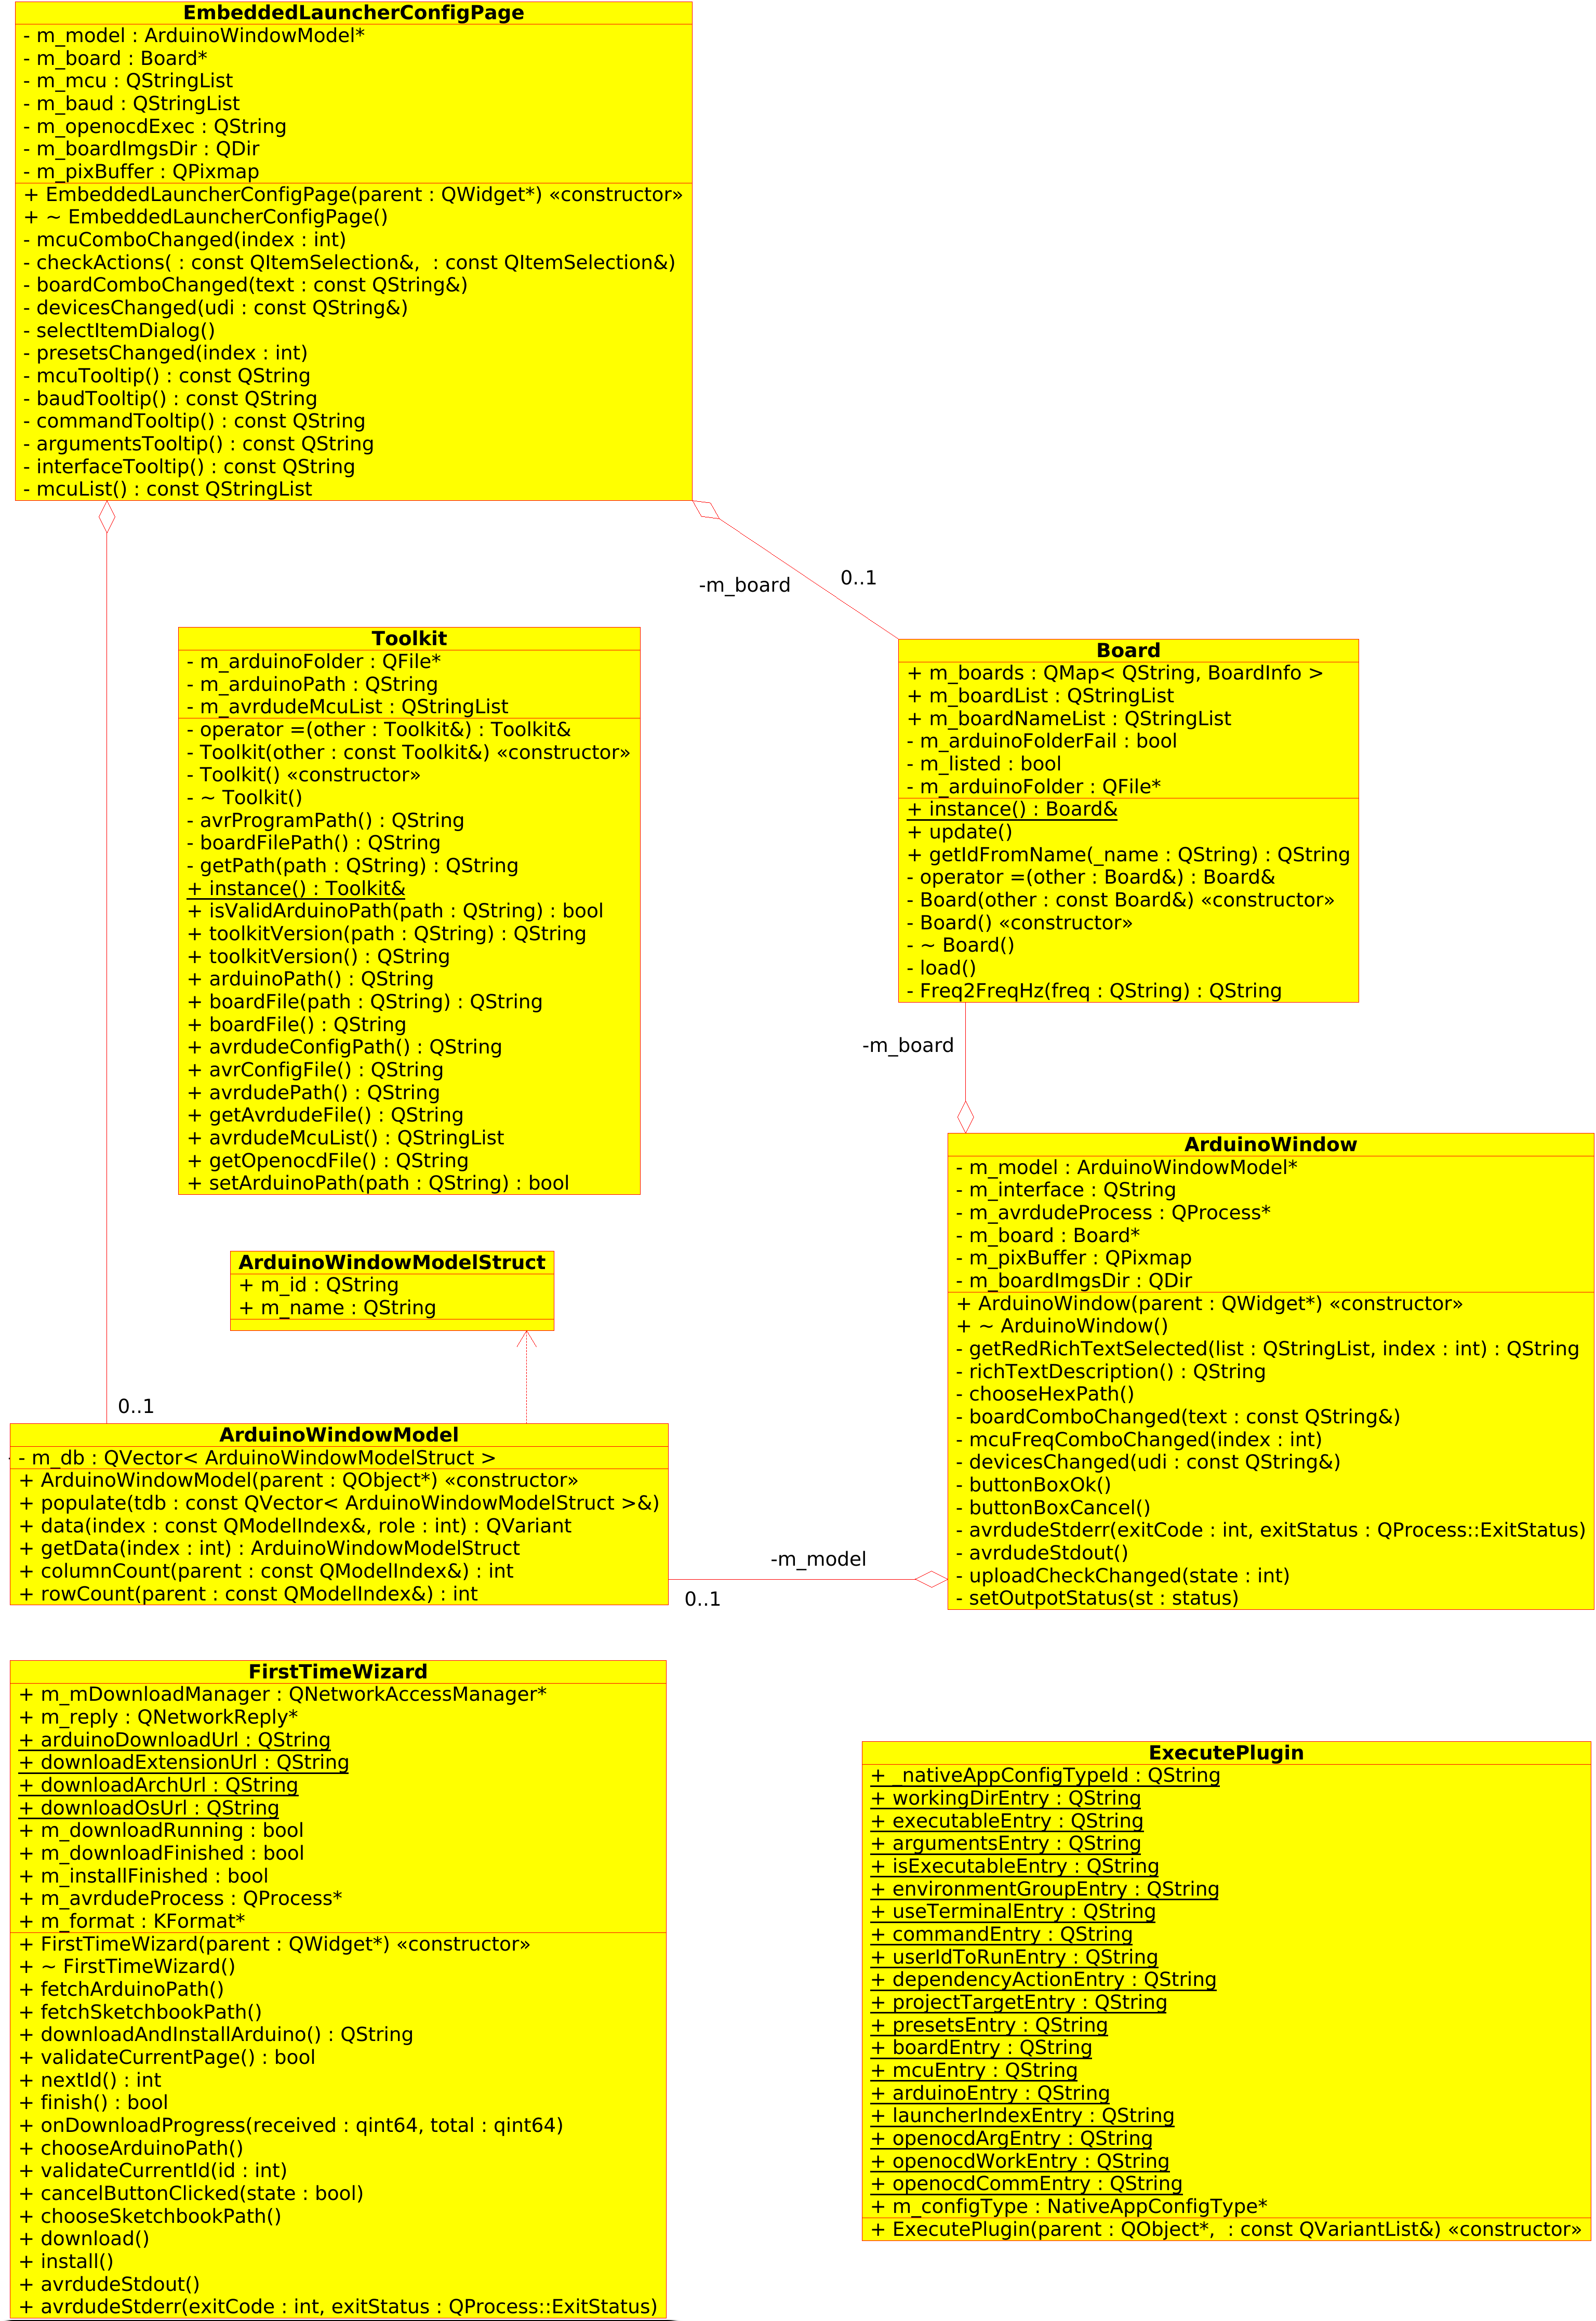
\includegraphics[width=0.85\textwidth]{figuras/uml.png}
  \caption[UML proposto]{UML proposto para desenvolvimento do plugin.}
  \label{fig:uml}
\end{figure}

\abreviatura{UML}{Unified Modeling Language}

O plugin (\figref{fig:uml}) foi integrado no KDevelop (\figref{fig:kdevelop}) via a utilização de ferramentas básicas de desenvolvimento para o mesmo (\textit{kdevplatform}). Nesta seção, será demonstrando as interfaces desenvolvidas e sua integração com o KDevelop.

\begin{figure}[!htb]
  \centering
  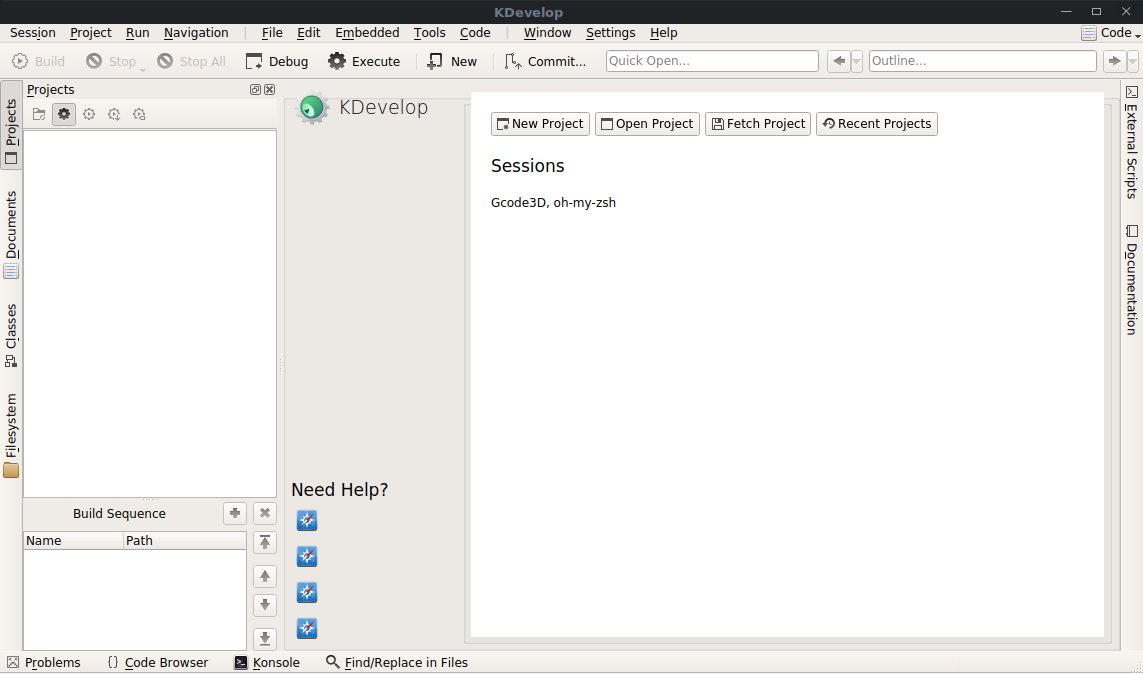
\includegraphics[width=0.85\textwidth]{figuras/kdevelop.png}
    \caption[KDevelop]{KDevelop.}
    \label{fig:kdevelop}
\end{figure}

\subsection{Menu de acesso}

O menu de acesso (\figref{fig:kdevelopMenu}), foi desenvolvido para realizar duas funções, configurar o plugin em relação as ferramentas necessárias para sua utilização com as placas da \textit{Arduino} (\textit{Arduino Setup}), e permitir a realização do carregamento de código desenvolvido para a placa, utilizando uma interface gráfica assistencialista (\textit{Board settings}).

\begin{figure}[!htb]
  \centering
  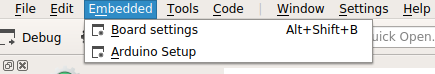
\includegraphics[width=0.95\textwidth]{figuras/kdevelopMenu.png}
  \caption[Menu do plugin no KDevelop]{Menu de acesso do plugin no KDevelop.}
  \label{fig:kdevelopMenu}
\end{figure}

\subsection{Arduino Setup}

Realiza a configuração inicial do plugin no sistema, permitindo ao usuário escolher uma versão do kit de ferramenta do \textit{Arduino} para utilizar ou a instalação automática do kit pelo plugin.

Primeiramente foi definido um diagrama inicial de estados para facilitar a compreensão da configuração (\figref{fig:ftwstate}).

\begin{itemize}
\item \textbf{\textit{First-Time Configuration} (FTC)}: Tela inicial, permitindo ao usuário escolher o local do \textit{toolkit} previamente instalado (\figref{fig:kdevelopinstaller1}), ou escolher a opção de instalação automática. 

\item \textbf{\textit{Automatic Instalation} (AutoInst)}: Tela resultante da escolha da instalação automática na configuração inicial do \textbf{\textit{First-Time Configuration}}. Essa, separada em duas etapas, \textit{Download} e \textit{Install}.

\subitem \textbf{\textit{Download} (Down)}: É realizado a comunicação com o servidor oficial resultando no download das ferramentas necessárias (\figref{fig:kdevelopinstaller21}).

\subitem \textbf{Install}: Após o \textit{download} é realizado a decomposição e instalação do conjunto de ferramentas (\figref{fig:kdevelopinstaller22}).

\item \textbf{\textit{End Configuration} (EndConf)}: Tela final, resulta após a escolha de um \textit{toolkit} previamente instalado ou após a conclusão da instalação automática (\figref{fig:kdevelopinstaller3}).
\end{itemize}

\begin{figure}[htb!]
  \centering
  \begin{tikzpicture}[->,>=stealth',shorten >=1pt,auto,node distance=2.8cm,semithick]
    \tikzstyle{every state}=[fill=blue,draw=none,text=white]

	%First-Time Configuration
    \node[state]         (A)                    {$FirstTimeConf.$}; 
    % Automactic Install
    \node[state]         (B) [right of=A]       {$Auto Inst.$};
    \node[state]         (C) [right of=B]       {$Down.$};
    \node[state]         (D) [below of=C]       {$Install$};
    \node[state]         (E) [below of=A]       {$EndConf$};

    \path (A) edge              node {Existing Installation}      (E)
	      (A) edge  [bend left]   node {Automatic Installation}      (B)
          (B) edge              node {}      (C)
          (C) edge              node {}      (D)
          (D) edge              node {}      (E);
  \end{tikzpicture}
  \caption[Diagrama de estados do \textit{First-Time Wizard}]{Diagrama de estados do \textit{First-Time Wizard}}
  {\label{fig:ftwstate}}
\end{figure}


\begin{figure}[!htb]
  \centering
  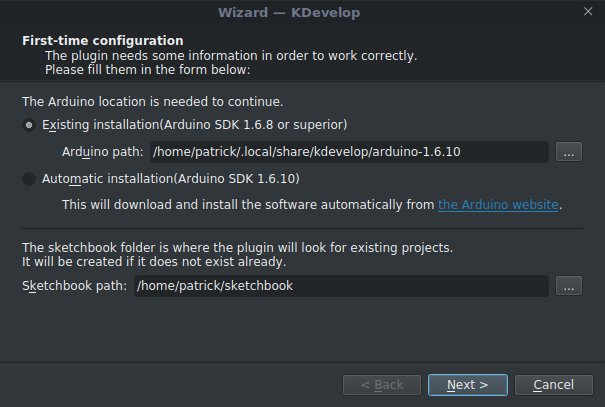
\includegraphics[width=0.85\textwidth]{figuras/kdevelopInstaller1.png}
  \caption[Fist-Time Configuration]{\textit{Fist-Time Configuration} com \textit{Existing Installation} selecionado.}
  \label{fig:kdevelopinstaller1}
\end{figure}

\begin{figure}[!htb]
  \centering
  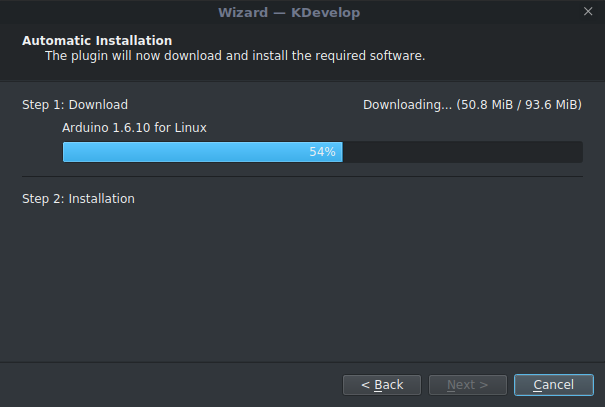
\includegraphics[width=0.85\textwidth]{figuras/kdevelopInstaller21.png}
  \caption[Automatic Instalation executando Download]{\textit{Automatic Instalation} com \textit{download} em andamento.}
  \label{fig:kdevelopinstaller21}
\end{figure}

\begin{figure}[!htb]
  \centering
  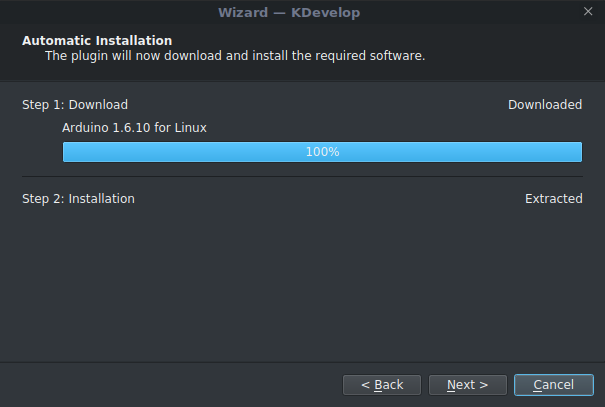
\includegraphics[width=0.85\textwidth]{figuras/kdevelopInstaller22.png}
  \caption[Automatic Instalation pós instalação]{Automatic Instalation após a instalação do \textit{toolkit}.}
  \label{fig:kdevelopinstaller22}
\end{figure}

\begin{figure}[!htb]
  \centering
  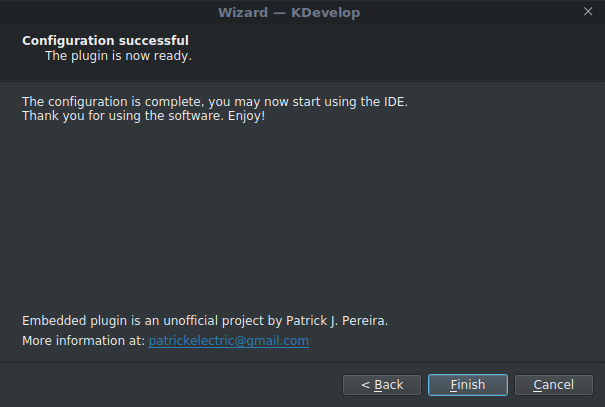
\includegraphics[width=0.85\textwidth]{figuras/kdevelopInstaller3.png}
  \caption[End Configuration]{End Configuration}
  \label{fig:kdevelopinstaller3}
\end{figure}

\subsection{Board Settings}

Interface para realizar o envio do binário para o sistema embarcado, permitindo o usuário interagir com o sistema, escolhendo a placa e algumas opções simples como processador, frequência, interface de comunicação, tipo de log de dados da saída do \textit{bootloader}. Além de permitir visualizar e mostrar quais opções foram selecionadas (\figref{fig:boardsettings}).

\begin{figure}[!htb]
  \centering
  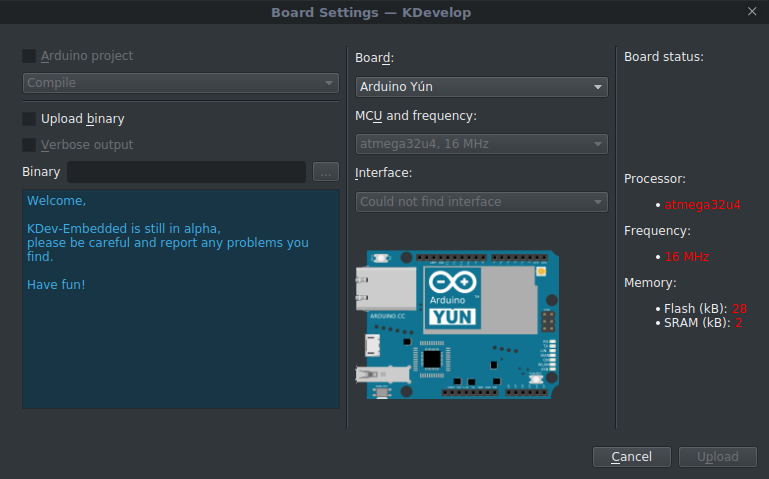
\includegraphics[width=0.85\textwidth]{figuras/boardsettings.png}
  \caption[Board Settings com configuração inicial]{\textbf{Board Settings} sem configuração prévia.}
  \label{fig:boardsettings}
\end{figure}

Após ter o acesso a interface, o usuário pode escolher a opção de \textit{Upload Binary}, selecionando desta forma um arquivo contendo o código de máquina (\textit{Blink.hex}), após isso, pode-se escolher no menu \textit{Board} a placa para programar, permitindo ao plugin selecionar as opções para o hardware indicado, além disso, é necessário selecionar o tipo de processador e clock, como consta no menu \textit{MCU and frequency}, tendo isto selecionado, a ultima configuração necessária para realizar o envio do código é a porta que consta no menu \textit{interface}. Essas configurações podem ser visualizadas na \figref{fig:boardsettingsserial}, onde foi escolhido um Arduino Nano contendo um processador atmega328p com um clock de $16MHz$ utilizando uma interface de programação \textit{FT232 USB UART}.

\begin{figure}[!htb]
  \centering
  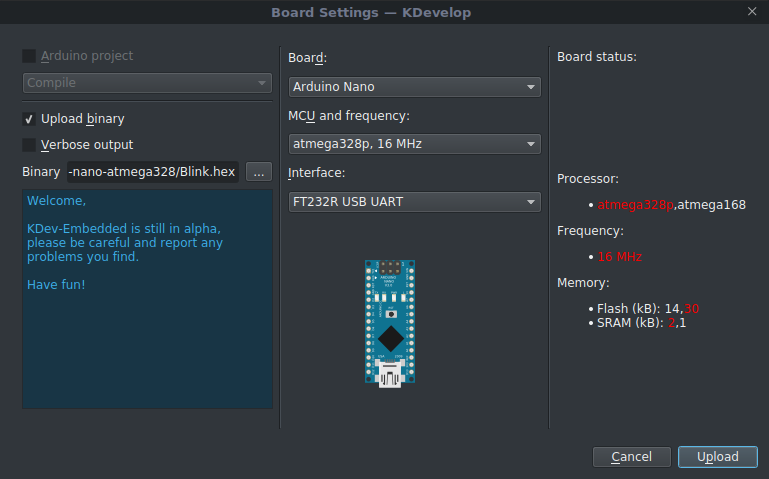
\includegraphics[width=0.85\textwidth]{figuras/boardsettingsSerial.png}
  \caption[Board Settings após configuração para envio]{\textbf{Board Settings} após configuração do usuário.}
  \label{fig:boardsettingsserial}
\end{figure}

Depois de tudo configurado, é possível clicar no botão \textit{upload} e realizar o envio do binário selecionado para placa. Podendo acarretar no sucesso da operação (\figref{fig:boardsettingsdone}) ou na sua falha (\figref{fig:boardsettingsndone}).

\begin{figure}[!htb]
  \centering
  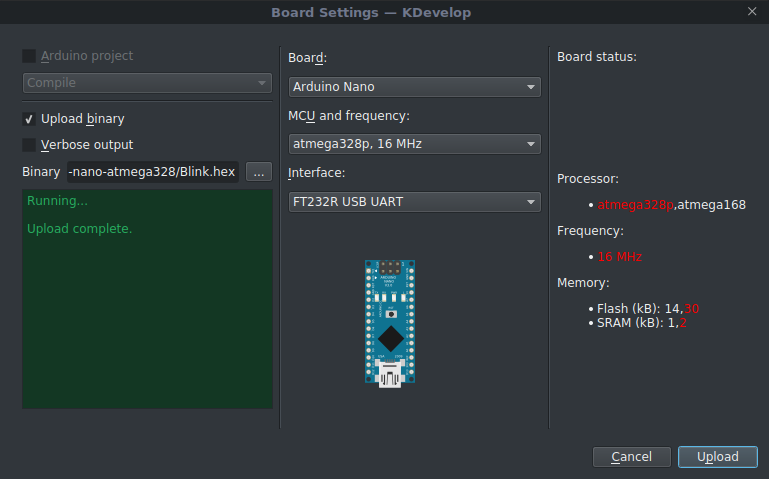
\includegraphics[width=0.85\textwidth]{figuras/boardsettingsdone.png}
  \caption[Board Settings com sucesso no envio]{\textbf{Board Settings} após o envio do código para o sistema embarcado.}
  \label{fig:boardsettingsdone}
\end{figure}

\begin{figure}[!htb]
  \centering
  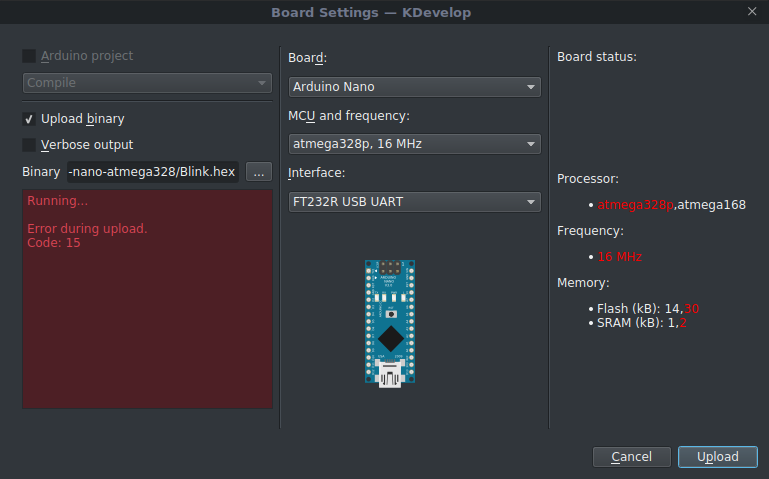
\includegraphics[width=0.85\textwidth]{figuras/boardsettingsndone.png}
  \caption[Board Settings com falha no envio]{Imagem do \textbf{Board Settings} após falha no envio do código para o sistema embarcado.}
  \label{fig:boardsettingsndone}
\end{figure}

\section{Integração com fluxo de trabalho}
Além do desenvolvimento do software, permitindo seu uso como projetado inicialmente, foi necessário reservar uma parte do período do projeto para modificações de interface gráfica e de organização de layout, permitindo um uso simplificando para usuários não tão avançados, e ao mesmo tempo uma flexibilidade aos usuários com conhecimento profundo do funcionamento do sistema, modificando e personalizando as opções fornecidas pelo ambiente gráfico, sem restringir o alto nível de abstração que essas ferramentas já permitem.

\subsection{Integração e compilação do projeto}

Para o usuário realizar a compilação, é necessário importar um projeto: Project $\rightarrow$ Open / Import Project... e importar um projeto com um sistema de compilação suportado pelo KDevelop, seguindo o fluxo de trabalho do KDevelop (\figref{fig:importproject}).

\begin{figure}[!htb]
  \centering
  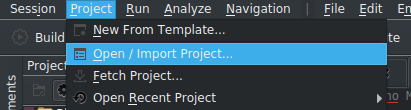
\includegraphics[width=1\textwidth]{figuras/importproject.png}
  \caption[Import Project]{Import Project.}
  \label{fig:importproject}
\end{figure}

Após o projeto ser importado com sucesso, será possível visualizar o mesmo no menu de projeto (\figref{fig:projects}).

\begin{figure}[!htb]
  \begin{minipage}[t]{0.5\textwidth}
  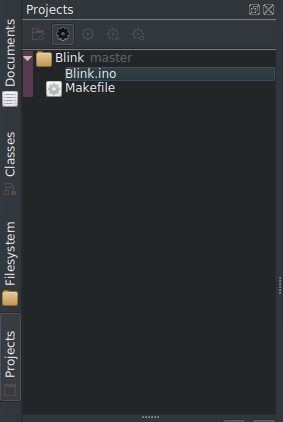
\includegraphics[width=0.7\textwidth]{figuras/projects.png}
  \caption[Projects antes da compilação]{Dock Projects antes\\ da compilação do projeto.}
  \label{fig:projects}
  \end{minipage}%
  \begin{minipage}[t]{0.5\textwidth}
%  \raggedleft
  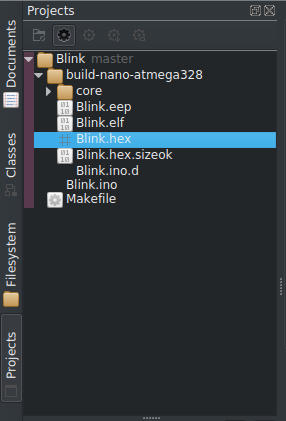
\includegraphics[width=0.713\linewidth]{figuras/projects2.png}
  \caption[Projects depois da compilação]{Dock Projects depois\\ da compilação do projeto.}
  \label{fig:projects2}
  \end{minipage}
\end{figure}

Depois de ter realizado a importação com sucesso, é necessário realizar a compilação para gerar o binário que será enviado para o processador, realizando o processo de compilação, basta clicar no botão \textit{Build} da interface do KDevelop, após isso, o menu de projeto se atualizado, podendo ser possível visualizar o arquivo com o código de máquina (\figref{fig:projects2}).

\subsection{Lançamento}

Seguindo o fluxo de trabalho do KDevelop, é necessário configurar o projeto para ser realizado o lançamento de uma forma correta. Para tal, basta executar Run $\rightarrow$ Configure Launchs (\figref{fig:run}).

\begin{figure}[!htb]
  \centering
  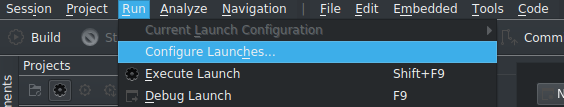
\includegraphics[width=1\textwidth]{figuras/run.png}
  \caption[Configure Launchs]{Configure Launchs.}
  \label{fig:run}
\end{figure}

Após isso, uma tela de configuração será aberta, podendo ser configurado da seguinte forma para um sistema embarcado, Add New... $\rightarrow$ Embedded e modificando o sistema de acordo com o alvo que será programado, \figref{fig:run2}. Nesta, foi utilizado um \textit{Arduino Nano} para realizar o teste de envio de código, também é possível selecionar a opção de \textit{OpenOCD} desenvolvido (\figref{fig:openocd}).

\begin{figure}[!htb]
  \centering
  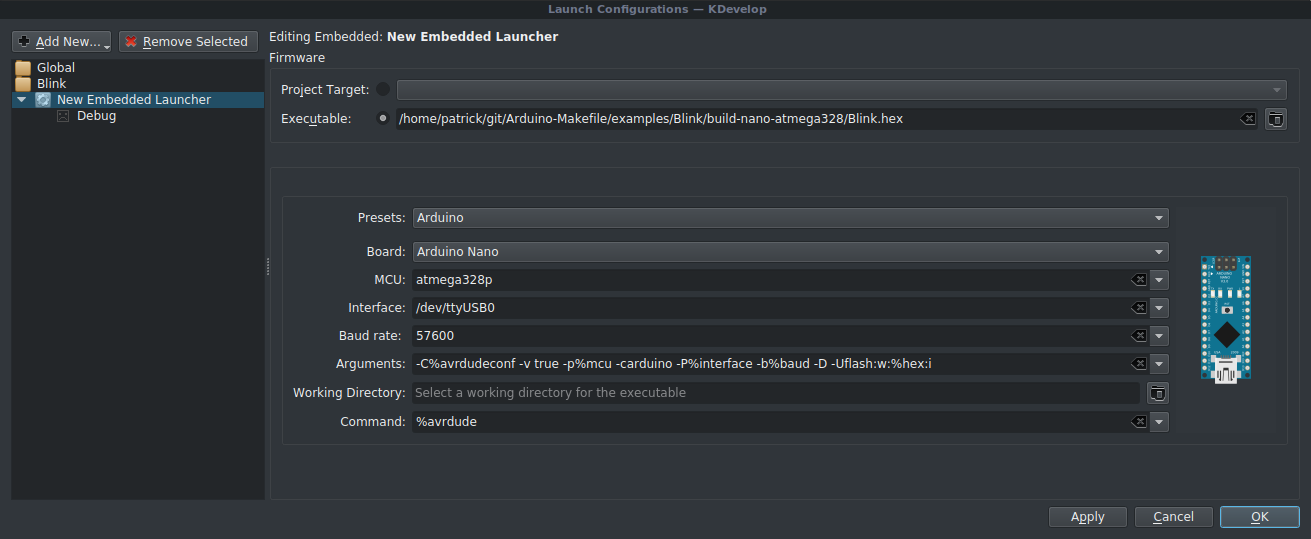
\includegraphics[width=1\textwidth]{figuras/run2.png}
  \caption[\textit{Configure Launchs} para \textit{avrdude}]{Configure Launchs para \textit{avrdude}.}
  \label{fig:run2}
\end{figure}

\begin{figure}[!htb]
  \centering
  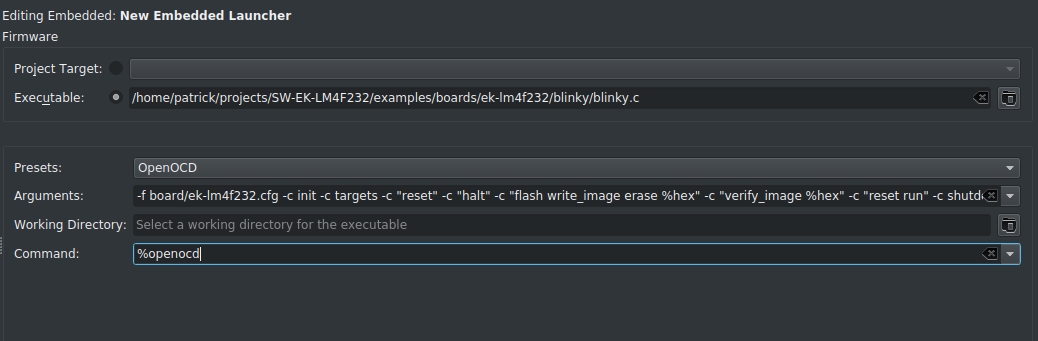
\includegraphics[width=1\textwidth]{figuras/openocd.png}
  \caption[\textit{Configure Launchs} para \textit{OpenOCD}]{Configure Launchs para \textit{OpenOCD}.}
  \label{fig:openocd}
\end{figure}

Após realizar as configurações, basta aplica-las e em seguida executar o lançamento com o botão Execute. Tendo isso realizado, será aberto um console onde todos os dados de gravação serão mostrados (\figref{fig:runavrdude} e \figref{fig:runopenocd}).

Com as configurações salvas no lançador do código, as mesmas ficam reservadas em um arquivo conhecido como *.kdev4, responsável por gerenciar os arquivos de configuração, permitindo que os próximos lançamento sempre utilizem as mesmas configurações, além de permitir outras configurações de lançamento em paralelo.

\begin{figure}[!htb]
  \centering
  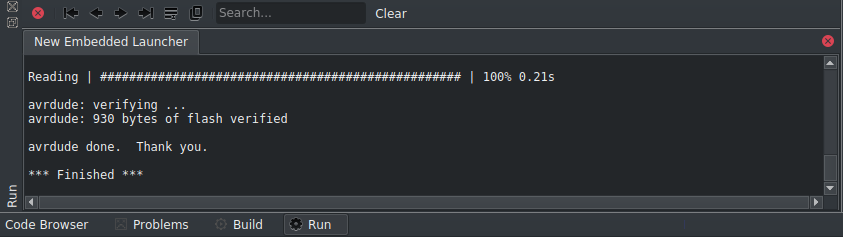
\includegraphics[width=1\textwidth]{figuras/runavrdude.png}
  \caption[\textit{Embedded Launcher} com \textit{avrdude}]{Embedded Launcher com saída do \textit{avrdude.}}
  \label{fig:runavrdude}
\end{figure}

\begin{figure}[!htb]
  \centering
  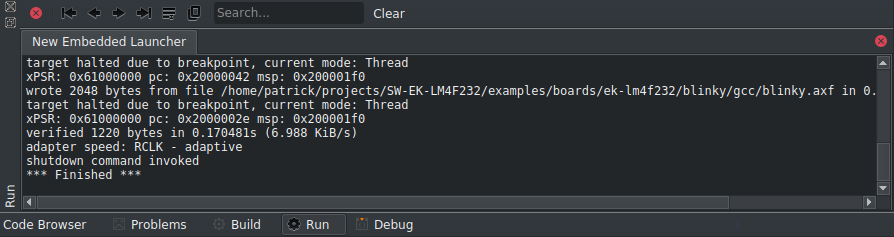
\includegraphics[width=1\textwidth]{figuras/runopenocd.png}
  \caption[\textit{Embedded Launcher} com \textit{openocd}]{Embedded Launcher com saída do \textit{openocd.}}
  \label{fig:runopenocd}
\end{figure}

\subsection{Depuração}

A depuração pode ser realizada utilizando as próprias ferramentas do KDevelop, permitindo uma conexão com o servidor do GDB pela porta padrão, tal configuração foi testada utilizando a implementação do \textit{OpenOCD} (\figref{fig:openocddebug}).

\begin{figure}[!htb]
  \centering
  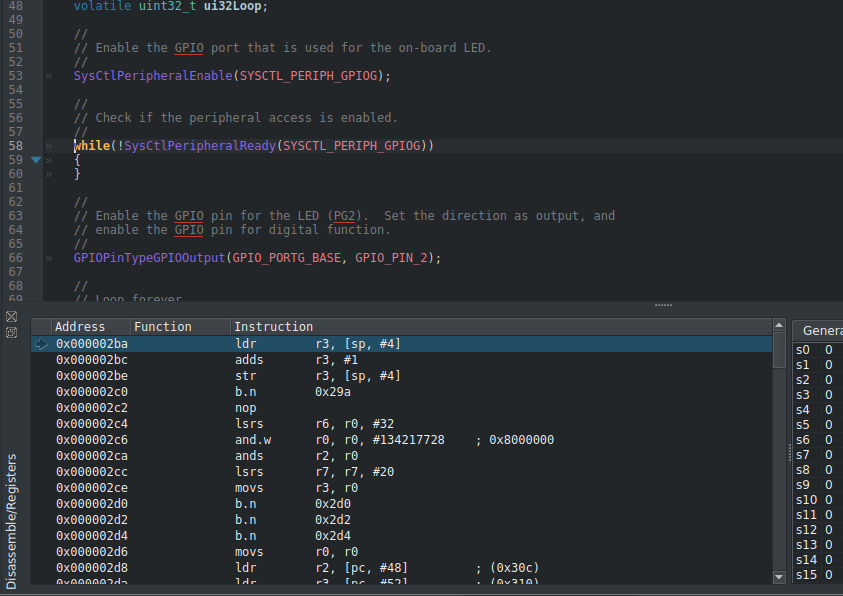
\includegraphics[width=0.85\textwidth]{figuras/DEBUG.png}
  \caption[\textit{Debug mode} com \textit{openocd} no KDevelop]{\textit{Debug mode} com \textit{openocd.} no KDevelop}
  \label{fig:openocddebug}
\end{figure}


\chapter{Experimento e Resultados}
Finalizada a fase de desenvolvimento da ferramenta, uma fase de testes foi iniciada com intuito de validar a ferramenta desenvolvida.

\section{Ambiente Experimental}

Todas as placas foram programas com o plugin desenvolvido utilizando um computador com o sistema operacional Linux, com o SDK do Arduino versão 1.6.10. A versão do KDevelop utilizado com o plugin foi a 5.0.0, contendo as atualizações da versão do QT 5.8 assim como uma boa parte do código migrado para C++11.

\subsection{Hardware Utilizado}

Os processos de gravação foram realizados via USB, por intermédio de um hardware especializado para realizar a gravação ou um adaptador serial-USB para permitir uma comunicação do software de programação para com o \textit{bootloader}.

O Arduino Mega possui um processador ATmega2560, com 10 entradas analógicas a mais que o Arduino UNO, com 54 pinos digitais, 15 com função de \textit{PWM} e contendo um grande vantagem em memória \textit{RAM} e \textit{EEPROM}.

\abreviatura{RAM}{\textit{Random Access Memory}}


O Arduino Nano Por ser uma placa de desenvolvimento completa, com um tamanho de aproximadamente um quarto do Arduino UNO, se tornou muito popular pela mobilidade e facilidade de desenvolvimento, assim como o \textit{pinout}\footnote{ Referencia utilizada para equidistância entre os pinos ou conexões.} ideal para ser encaixado numa \textit{protoboard}\footnote{Matriz de contato, utilizada para realizar ensaios de circuitos, contem contatos e conexões para montagem.}. Além disso, alguns modelos tem dois pinos a mais de entrada analógica comparado com o Arduino Pro Mini e Arduino UNO.

Desenvolvido para aplicações com pouco espaço e para instalações permanentes, o Arduino pro mini utiliza um processador ATmega328,  diferente de outras placas da Arduino, está não possui um hardware assistencialista para a realização do \textit{upload} do processador na própria placa, logo, tal artefato, necessita ser conectado na placa para realizar a sua programação, apesar disso, contem as demais características do Arduino UNO.

Sendo a placa de desenvolvimento de lançamento comemorativa do lançamento oficial do arduino, o Arduino UNO utiliza o processador ATmega328P, sendo a primeira que utiliza USB para realizar o \textit{upload} do código de maquina para o processador via \textit{bootloader}. Contem 6 entradas analógicas, 14 pinos digitais, 6 pinos de \textit{PWM}, 1kb de \textit{SRAM}, 2kb de \textit{EEPROM}, 32kb de flash e 1 serial em hardware. Muito similar ao Arduino Nano, porém, conta com duas portas analógicas a menos.

\abreviatura{SRAM}{\textit{{Static Random Access Memory}}}
\abreviatura{EEPROM}{\textit{Electrically-Erasable Programmable Read-Only Memory}}

ARM é uma arquitetura baseada na família RISC de processadores, onde as instruções tendem a ser operações simples, onde as mais complexas são quebradas até chegar em instruções uno.

Atualmente é considera a arquitetura mais popular entre sistemas computacionais após a revolução \textit{mobile} dos telefones e \textit{smartphones}.

Muitas placas de desenvolvimento, tanto para profissionais quanto para hobbistas possuem processadores ARM ou variantes que utilizam este mesmo processador, tanto para usos em \textit{bere-metal} quanto para usos com sistema operacional.

\abreviatura{RISC}{\textit{Reduced Instruction Set}}

O STM32 se trata de uma família de processadores da arquitetura ARM de 32-bits pertencentes a empresa STMicroelectronics. O Cortex-M, cerne do processador, pode ser encontrado em alguns processadores conhecidos como: Cortex-M0, Cortex-M1, Cortex-M3, Cortex-M4, Cortex-M7 entre outros. Sendo todos distintos pelo hardware de suporte a CPU, podendo ter FPU, decodificação de instruções de DSP, eficiência energética e etc.

\abreviatura{FPU}{\textit{Float Point Unit}}
\abreviatura{DSP}{\textit{Digital Signal Processing}}
%\itodo{Adicionar fotos da placa}

\section{Testes Realizados}

Inicialmente foram avaliados alguns modelos de Arduíno, entre as versões atuais, as utilizadas foram: Arduino nano, Arduino Mini e Arduino Mega.

Para demonstrar o funcionamento minimo do sistema, foi utilizado o projeto Arduino-Makefile\footnote{\url{https://github.com/sudar/Arduino-Makefile}} com o exemplo de piscar o LED (Algoritmo 6.1) em todas as placas da Arduino.

\lstinputlisting[language=C++,caption={blink.ino},label=blink]{blink.ino}

O código foi compilado e enviado para todas as placas, executando o código de piscar o LED.

No teste do \textit{OpenOCD}, foi utilizado um projeto exemplo de piscar o LED da placa de desenvolvimento STM32F4DISCOVERY (Algoritmo 6.2)

\lstinputlisting[language=C++,caption={project.c},label=blink2]{blink2.cpp}

O Código foi compilado e enviado para a placa, tendo como resultado o piscar do LED.

\chapter{Conclusão}
Dentro do período de desenvolvimento, o plugin alcançou todas as expectativas traçadas para o período de desenvolvimento,
permitindo a gravação dos sistemas embarcados utilizando o KDevelop, mesmo necessitando algumas modificações para ficar
totalmente integrado ao fluxo de trabalho.

A integração com o KDevelop foi realizada com sucesso, necessitando que o usuário configure algumas variáveis para permitir identificar o hardware utilizado pelo mesmo, tanto o processador quanto o hardware especialista ou assistencialista na realização do envio do código binário.

O código fonte do projeto desenvolvido pode ser encontrado no \textit{mirror} do \textit{GitHub} (\url{https://github.com/KDE/kdev-embedded/tree/master}) ou no repositório oficial do \textit{phabricator} (\url{https://phabricator.kde.org/source/kdev-embedded/browse/master/}).

Tendo em vista que com o suporte para as placas da \textit{Arduino} e do sistema \textit{OpenOCD} realizado, ainda é necessário mais alguns trabalhos relacionados a áreas especificas.

As interfaces desenvolvidas foram trabalhadas para serem a mais ami-gáveis e altamente configuráveis na medida do possível, contudo, ainda é necessário um polimento e melhor desenvolvimento tanto da interface do plugin quanto do KDevelop, para permitir uma melhor integração com o usuário, facilitando algumas configurações básicas como a já existentes no \textit{eclipse IDE} para \textit{debug} remoto.

Mesmo o instalador sendo completamente funcional, identificando ver-sões instaladas no sistema operacional e
permitindo ao usuário realizar a instalação automática das dependências, com a ajuda da interface gráfica disponível pelo plugin, o mesmo não é de muita ajuda para os usuários avançados.

A integração do plugin desenvolvido com os demais plugins do KDevelop necessita ser melhor integrado e aprimorada, permitindo desta
forma a integração com os gerenciadores de montagem de software.

Atualmente o plugin utiliza uma biblioteca desenvolvida pela comunidade do KDE conhecida como \textit{Solid}, onde permite uma boa integração com o \textit{hardwre} do computador onde o mesmo está sendo executado. Contudo o mesmo tem problemas para identificação de gravadores que não utilizam um adaptador Adaptador Serial-USB, dificultando sua utilização. 

Como proposta de solução, é utilizar os valores de PID e VID dos dispositivos conhecidos na realização da gravação, podendo ser obtidos através das bibliotecas do \textit{OpenOCD}, para melhorar sua utilização na detecção de hardware.

\abreviatura{PID}{\textit{Product ID}}
\abreviatura{VID}{\textit{Vendor ID}}


\bibliographystyle{ufscThesis/ufsc-alf}
\bibliography{bibliografia}

%--------------------------------------------------------
% Elementos pós-textuais
\apendice
\chapter{Exemplificando um Apêndice}
Texto do Apêndice aqui. 

\anexo
\chapter{Exemplificando um Anexo}
Texto do anexo aqui.
\end{document}
